\chapter{Corpus}
\label{chp:corpus}

This chapter is based on the following publication.

\begin{infobox-pub}
\fullcite{Saier2020}
\end{infobox-pub}
\vspace{-0.5em}
\begin{footnotesize}
\textit{Remark on the connection to previous work:}
\vspace{-0.5em}
\begin{quote}
The publication cited above is a journal article that represents an extension of a previously published workshop paper~\cite{Saier2019} (see also Table~\ref{tab:secondarypublicationoverview}). For the journal article, the underlying work, writing, and publication were conducted within the doctoral research period. The preceding workshop paper reports on a result of the master's thesis before the doctoral research period (see also Section~\ref{sec:intro-puboverview}). Later in this chapter, at the end of Section~\ref{sec:related-work}, further details regarding the nature of the extension are provided.
\end{quote}
\end{footnotesize}

The work in this chapter addresses the following research task.

\begin{rtlist}
    \item \textit{Base Methodology} - identify or establish a base methodology for generating a large-scale, high quality scholarly data set, that is on par with or improving upon existing data sets.
\end{rtlist}

It furthermore makes contributions to the following research task, which is likewise addressed in the next chapter.

\begin{rtlist}
    \item[\rtmark{2}:] \textit{Citation Network Completeness} - develop a method to link literature references, that is able to link more references than are linked in existing data sets, while not compromising on link correctness or processing efficiency.
\end{rtlist}

\section{Overview}
In this chapter, we introduce a methodology for creating a large-scale corpus of linked, full-text documents from \LaTeX\ source files. The resulting corpus, \emph{unarXive}, comprises over one million documents across multiple scientific disciplines, and spans 27 years. It is further on also used as the basis for the research presented in the subsequent chapters. Along with the corpus creation methodology, extensive analyses of the resulting corpus are presented.

At the end of the chapter in Section~\ref{sec:corpus-assessment}, we assess the achievement of the research tasks, as well as the contributions made in terms of the overarching research goal of enabling higher-quality scholarly data.

% \begin{abstract}
% In recent years, scholarly data sets have been used for various purposes, such as paper recommendation, citation recommendation, citation context analysis, and citation context-based document summarization. 
% The evaluation of approaches to such tasks and their applicability in real-world scenarios heavily depend on the used data set. However, existing scholarly data sets are limited in several regards. 
% In this paper, we propose a new data set based on all publications from all scientific disciplines available on arXiv.org. Apart from providing the papers' plain text, in-text citations were annotated via global identifiers. Furthermore, citing and cited publications were linked to the Microsoft Academic Graph, providing access to rich metadata. Our data set consists of over one million documents and 29.2 million citation contexts. The data set, which is made freely available for research purposes, not only can enhance the future evaluation of research paper-based and citation context-based approaches, but also serve as a basis for new ways to analyze in-text citations, as we show prototypically in this chapter.
% \end{abstract}

\section{Introduction}
A variety of approaches exist that utilize scientific paper collections to help researchers in their work. 
Research paper recommender systems, for example, suggest relevant papers to read~\cite{Beel2016fixed}. Other systems operate on a more fine-grained level within the full-text of papers, such as the textual contexts in which citations appear (i.e., citation contexts). 
Based on citation contexts, things like the citation function~\cite{Teufel2006EMNLP,Teufel2006fixed,Moravcsik1975}, the citation polarity~\cite{GhoshD017,Abu-Jbara2013fixed}, and the citation importance~\cite{Valenzuela2015fixed,Chakraborty2016} can be determined. Furthermore, citation contexts are necessary for context-aware citation recommendation~\cite{He2010WWW,Ebensu2017}, as well as for citation-based document summarization tasks~\cite{Chandrasekaran2019}, such as citation-based automated survey generation~\cite{Mohammad2009} and automated related work section generation~\cite{Jinggiang2007}.

The evaluation such approaches approaches, as well as the actual applicability and usefulness of developed systems in real-world scenarios, heavily depend on the data that is used. This typically is a collection of papers provided as full-text, or a set of already extracted citation contexts, consisting of, for instance, 1--3 sentences each. Existing data sets, however, do not fulfill all of the following criteria (see Sec.~\ref{sec:related-work} for more details):
\begin{enumerate}
 \item \textit{Size.} The data set can be comparatively small (below 100,000 documents) which makes it difficult to use it for training and testing machine learning approaches; 
 \item \textit{Cleanliness.} The papers' full-texts or citation contexts are often very noisy due to the conversion from PDF to plain text and due to encoding issues;
 \item \textit{Global citation annotations.} No links from the citations in the text to the structured representations of the cited publications across documents are provided;
 \item \textit{Data set interlinkage.} Data sets often do not provide identifiers of the citing and cited documents from widely used bibliographic databases, such as DBLP\refurl{https://dblp.uni-trier.de/}{2023-11-06} or the Microsoft Academic Graph (MAG)\refurl{https://www.microsoft.com/en-us/research/project/microsoft-academic-graph/}{2023-11-06};
 \item \textit{Cross-domain coverage.} Often, only a single scientific discipline is available for evaluating or applying an approach to a paper or citation-based task.
\end{enumerate}

To address these limitations, we propose a new scholarly data set, which we call \emph{unarXive}.\footnote{The name is derived from the name of the data source, \textit{arXiv}, and the verb \textit{to unarchive}, indicating the extraction of files from an archive.} The data set comprises papers' full-text, a citation network, and additional metadata.
It is freely available \refurlinline{http://doi.org/10.5281/zenodo.3385851}{2023-11-06} and the implementation for creating it at \refurlinline{https://github.com/IllDepence/unarXive}{2023-11-06}.

\begin{table}[t]
\centering
  \caption{Overview of the proposed data set}
  \label{tbl:allthestats}
\begin{small}
\begin{tabular}{lrcc|cc}
\toprule
    \ & \ & citing & \ & \ & cited \\
    \ & \ & documents & \multicolumn{2}{c}{references} & documents \\
    \ & \ & \  & \tiny{outgoing} & \tiny{incoming} & \  \\
    \emph{full data set:} & \ & \textbf{1,043,126} & 15,954,664 & 15,954,664 & \textbf{2,746,288} \\
    &\tiny{full-text}&\tiny{1,043,126}&\tiny{15,954,664}&\tiny{7,181,576}&\tiny{736,597}\\
    &\tiny{linked to MAG}&\tiny{994,351}&\tiny{15,846,351}&\tiny{15,954,664}&\tiny{2,746,288}\\
    \emph{by discipline:} & \ & \ & \ & \ & \ \\
    \multicolumn{2}{r}{physics} & 662,894 & 9,300,576 & 7,827,072 & 921,852 \\
    \multicolumn{2}{r}{mathematics} & 237,422 & 3,426,117 & 5,062,033 & 906,301 \\
    \multicolumn{2}{r}{computer science} & 111,694 & 2,526,656 & 1,876,401 & 425,860 \\
    \multicolumn{2}{r}{other} & 31,116 & 701,315 & 1,189,158 & 492,275 \\
  \bottomrule
    \\
    \multicolumn{6}{l}{
        \begin{tabular}{rl}
            \textbf{data}: & \refurlinline{http://doi.org/10.5281/zenodo.3385851}{2023-11-06} \\
            \textbf{code}: & \refurlinline{https://github.com/IllDepence/unarXive}{2023-11-06} \\
        \end{tabular}
        }
\end{tabular}
\end{small}
\end{table}

Table \ref{tbl:allthestats} gives an overview of the proposed data set. Note that throughout this chapter, we refer to links between publications on the \emph{document level} as ``references'' (corresponding to entries in a section ``bibliography'' or ``references'' near the end of a document), whereas on the \emph{text level} we speak of ``citations'' (indicated by markers within the text associated with a reference). The proposed data set consists of over one million full-text documents (about 269 million sentences) and links to 2.7 million unique publications via 15.9 million unique references and 29.2 million citations.
Thus, we argue that it is considerably large, fulfilling criterion (1). By using publications' \LaTeX{} source files and developing a highly accurate transformation method that converts \LaTeX{} to plain text, we can resolve issue (2). Besides the pure papers' content, in-text citations are annotated directly in the text via global identifiers, thereby covering aspect (3). As far as possible, (citing and cited) documents are linked to the Microsoft Academic Graph \cite{Sinha2015MAG} (cf. item (4)). This enables us to use the arXiv paper content in combination with the metadata in the MAG, which, as of February 2019, contains data on 213 million publications along with metadata about researchers, venues, and fields of study. Our data set also fulfills constraint (5) as all disciplines covered in arXiv are included. This enables researchers to analyze papers from several disciplines and to compare approaches using scholarly data across disciplines.

% Aspect/benefit #1:
Considering the application of our data set, we argue that it not only can be used as a new large data set for evaluating paper-based and citation-based approaches with unlimited citation context lengths (since the publications' full-text is available),
% Aspect/benefit #2:
but also be a basis for novel ways of paper analytics within bibliometrics and scientometrics. For instance, based on the citation contexts and the citing and cited papers' metadata in the MAG, analyses on biases in the writing and citing behavior of researchers---e.g. related to authors' affiliation~\cite{Reingewertz2018} or documents' language~\cite{Liang2013,Liu2018}---can be performed.
%% Aspect/benefit #3:
Furthermore, (sophisticated) deep learning approaches, as they are also widely used in the digital library domain recently \cite{Ebensu2017}, require huge amounts of training data. Our data set allows to overcome this hurdle and investigate how far deep learning approaches can lead us.
% overall
Overall, we argue that with our data set we can significantly bring the state of the art of big scholarly data one step forward.

We make the following contributions in this chapter:
\begin{enumerate}
    \item We propose a large, interlinked scholarly data set with papers' full-text, annotated in-text citations, and links to rich metadata. We describe its creation process in detail and provide both the data as well as the creation process implementation to the public. 
    \item We manually evaluate the validity of our reference links on a sample of 300 references, thereby providing insight into our citation network's quality.
    \item We calculate statistical key figures and analyze the data set with respect to its contained references and citations.
    \item We compare our reference links to those in the MAG, and manually evaluate the validity of links only appearing in either of the data sets. In doing so, we identify a large number of documents where the MAG lacks coverage.
    \item We analyze the likelihood with which in-text citations in our data set refer to specific parts of a cited document depending on the discipline of the citing \emph{and} cited document. Such an analysis is only possible with word level precision citation marker positions annotated in full-text \emph{and} metadata on citing as well as cited documents. The analysis therefore can showcase the practicability of our data set.
\end{enumerate}

The remainder of the chapter is structured as follows: After outlining related data sets in Section~\ref{sec:related-work}, we describe in Section~\ref{sec:data-set-creation} how we created our data set. This is followed by statistics and key figures in Section~\ref{sec:statistics}. In Section~\ref{sec:evaluation-validity-and-coverage}, we evaluate the validity and coverage of our reference links. Section~\ref{sec:analysis} is dedicated to the analysis of the citation flow and the contexts within our data set. We conclude in Section~\ref{sec:conclusion} with a summary and an outlook.

\section{Existing Data Sets}
\label{sec:related-work}

Table~\ref{tab:existing-data-sets} gives an overview of related data sets.
CiteSeerX can be regarded as the most frequently used evaluation data set for citation-based tasks.
For our investigation, we use the snapshot of the entire CiteSeerX data set as of October 2013, published by~\cite{Huang2015fixed}. This data set consists of 1,017,457 papers, together with 10,760,318 automatically extracted citation contexts.
This data set has the following drawbacks \cite{Roy2016fixed,Faerber2018LREC}: The provided meta-information about cited publications is often not accurate. Citing and cited documents are not interlinked to other data sets. Moreover, the citation contexts can contain noise from non-ASCII characters, formulas, section titles, missed references and/or other ``unrelated'' references, and do not begin with a complete word.

\begin{table}[tb]
 % \caption{Overview of existing data sets\\\small{(\#P.=Number of papers; Cit.\ cont.=Citation contexts; Ref.\ IDs=Reference IDs; CS=Computer Science, BM=Biomedicine, LS=Life Sciences, CL=Computer Linguistics)\\(\emph{extractable*} indicates that extraction might be error-prone due to papers only being available in PDF format)}}
 % NOTE: above is original caption, but does not compile in this document class
 \caption[Overview of existing data sets]{Overview of existing data sets (\#Papers=Number of papers; Cit.\ contexts=Citation contexts; CS=Computer Science, BM=Biomedicine, LS=Life Sciences, CL=Computer Linguistics; extractable* indicates that extraction might be error-prone due to papers only being available in PDF format)}
 \label{tab:existing-data-sets}
  \centering
  \begin{small}
 \begin{threeparttable}
 \begin{tabular}{llllll}
 \toprule
   Data set & \#\,Papers & Cit. contexts & Scope & Full text & Reference IDs \\
   \midrule
   % capital Ms and lowercase ks (supposed to be like that)
   CiteSeerX \cite{Caragea2014}/RefSeer \cite{Huang2015fixed} &  1.0\,M & 400 characters & (all) & no & no \\
   PubMed Central OAS\tnote{a} & 2.3\,M & extractable & BM/LS & yes & mixed \\
   Scholarly Dataset 2 \cite{Sugiyama2015} & 0.1\,M & extractable* & CS & yes & no \\
   arXiv CS \cite{Faerber2018LREC}   &  0.09\,M & 1 sentence & CS & yes & DBLP \\
   ACL-ARC \cite{Bird2008ACLARC} & 0.01\,M & extractable* & CS/CL & yes & no \\
   ACL-AAN \cite{Radev2013} & 0.02\,M & extractable* & CS/CL & yes & no  \\
   \bottomrule
 \end{tabular}
 \begin{tablenotes}
    \item[a] See \refurlinline{https://www.ncbi.nlm.nih.gov/pmc/tools/openftlist/}{2023-11-06}.
  \end{tablenotes}
\end{threeparttable}
  \end{small}
\end{table}

The PubMed Central Open Access Subset is another large data set that has been used for citation-based tasks~\cite{Gipp2015,Duma2016,Galke2018}. Contained publications are already processed and available in the JATS~\cite{Huh2014} XML format. While the data set overall is comparatively clean, heterogeneous annotation of citations within the text and mixed usage of identifiers of cited documents (PubMed, MEDLINE, DOI, etc.) make it difficult to retrieve high quality citation interlinkings of documents from the data set\footnote{To be more precise, the heterogeneity makes the usage of the data set \emph{as is} unfeasible. Resolving references to a single consistent set of identifiers retroactively would be an option, but comparatively challenging in the case of PubMed, because of the frequent usage of special notation in publication titles; see also: \refurlinline{https://zenodo.org/records/3598421/files/CITREC_Parser_Documentation.pdf}{2023-11-06}.}~\cite{Gipp2015}.

Beside the aforementioned, there are other collections of scientific publications. Among them are the ACL Anthology corpus \cite{Bird2008ACLARC} and Scholarly Dataset 2 \cite{Sugiyama2015}.
Note that these data sets only contain the publications themselves, typically in PDF format. Therefore, using such data sets for paper-based or citation-based approaches is troublesome, since one must preprocess the data (i.e., (1) extract the content without introducing too much noise, (2) specify global identifiers for cited papers, and (3) annotate citations with those identifiers).
Furthermore, there are data sets for evaluating paper recommendation tasks, such as CiteULike\refurl{https://web.archive.org/web/20190211033621/http://www.citeulike.org/faq/data.adp}{2023-11-06} or Mendeley,\refurl{https://data.mendeley.com/}{2023-11-06}. These, however, only provide metadata about publications or are not freely available for research purposes.

F{\"{a}}rber et al.\ also published a data set with annotated arXiv papers' content in the past~\cite{Faerber2018LREC}. In comparison, our data set is superior to it in the following regards:
\begin{enumerate}
    \item Our data set is considerably larger (1 M instead of 90 k documents).
    \item Our data set ensures cleanliness of the papers' full-text and citation contexts by using a more feature rich conversion pipeline.
    \item A new method for resolving references to consistent global identifiers has been developed. Contrary to the method in~\cite{Faerber2018LREC}, our method has been evaluated and performs very well (see Sec.~\ref{sec:evaluation-reference-resolution}).
    \item While~\cite{Faerber2018LREC} link documents solely to DBLP, which covers computer science papers, our data set links documents to the Microsoft Academic Graph, which covers all scientific disciplines and which has been used frequently in the digital library domain in recent years \cite{Mohapatra2019}.
    \item While the data set in~\cite{Faerber2018LREC} is restricted to computer science, the new data set covers all domains of arXiv (see Sec.~\ref{sec:statistics} and Fig.~\ref{fig:sankey}).
\end{enumerate}

Lastly, compared to a preliminary version of our data set~\cite{Saier2019}, the data we present here has been improved in several ways. Most notably, while in the initial version, only citing papers were associated with arXiv identifiers and only cited papers had been linked to the MAG, we now provide both types of IDs for both sides. This means, that for nearly all documents, MAG metadata is easily accessible, and full-text is not only available for all citing papers but now also for over a quarter of the cited papers. Moreover, we provide significantly more details and insights into the data set's creation process (see Section~\ref{sec:data-set-creation}) and its resulting characteristics (see Sections~\ref{sec:evaluation-validity-and-coverage} and \ref{sec:analysis}).



\section{Data Set Creation}
\label{sec:data-set-creation}

Scientific publications are usually distributed in formats targeted at \emph{human consumption} (e.g., PDF) or, in cases like arXiv, also as source files the aforementioned (e.g., \LaTeX{} sources for generating PDFs). Citation-based tasks, such as context-aware citation recommendation, in contrast, require \emph{automated processing} of the publications' textual contents as well as the documents' interlinking through in-text citations. The creation of a data set for such tasks therefore encompasses two main steps: extraction of plain text and resolution of references. In the following, we will describe how we approached these two steps using arXiv publications' \LaTeX{} sources and the Microsoft Academic Graph.

\subsection{Used Data Sources}
The following two resources are the basis of the data set creation process.

\paragraph{arXiv} hosts over 1.5 million documents from August 1991 onward.%
\refurl{https://arxiv.org/stats/monthly_submissions}{2023-11-06} They are available not only as PDF, but (in most cases) also as \LaTeX{} source files. The discipline most prominently represented is physics, followed by mathematics, with computer science seeing a continued increase in percentage of submissions ranking third (see Fig.~\ref{fig:sankey}). The availability of \LaTeX{} sources makes arXiv documents particularly well suited for extracting high quality plain text and accurate citation information. So much so, that it has been used to generate ground truths for the evaluation of PDF-to-text conversion tools~\cite{Bast2017}.
\paragraph{Microsoft Academic Graph} is a very large, automatically generated data set on 213 million publications, related entities (authors, venues, etc.), and their interconnections through 1.4 billion references.\footnote{Numbers as of February 2019.} It has been widely used as a repository of all publications in academia in the fields of bibliometrics and scientometrics \cite{Mohapatra2019}. While pre-extracted citing sentences are available, these do not contain annotated citation marker positions. Full text documents are also not available. The size of the MAG makes it a good target for matching reference strings\footnote{I.e., the entries in the reference section of a publication. See Lst.~\ref{lst:refitems} for examples.} against it, especially given that arXiv spans several disciplines.

\subsection{Pipeline Overview}

\begin{figure}[tb]
  \centering
    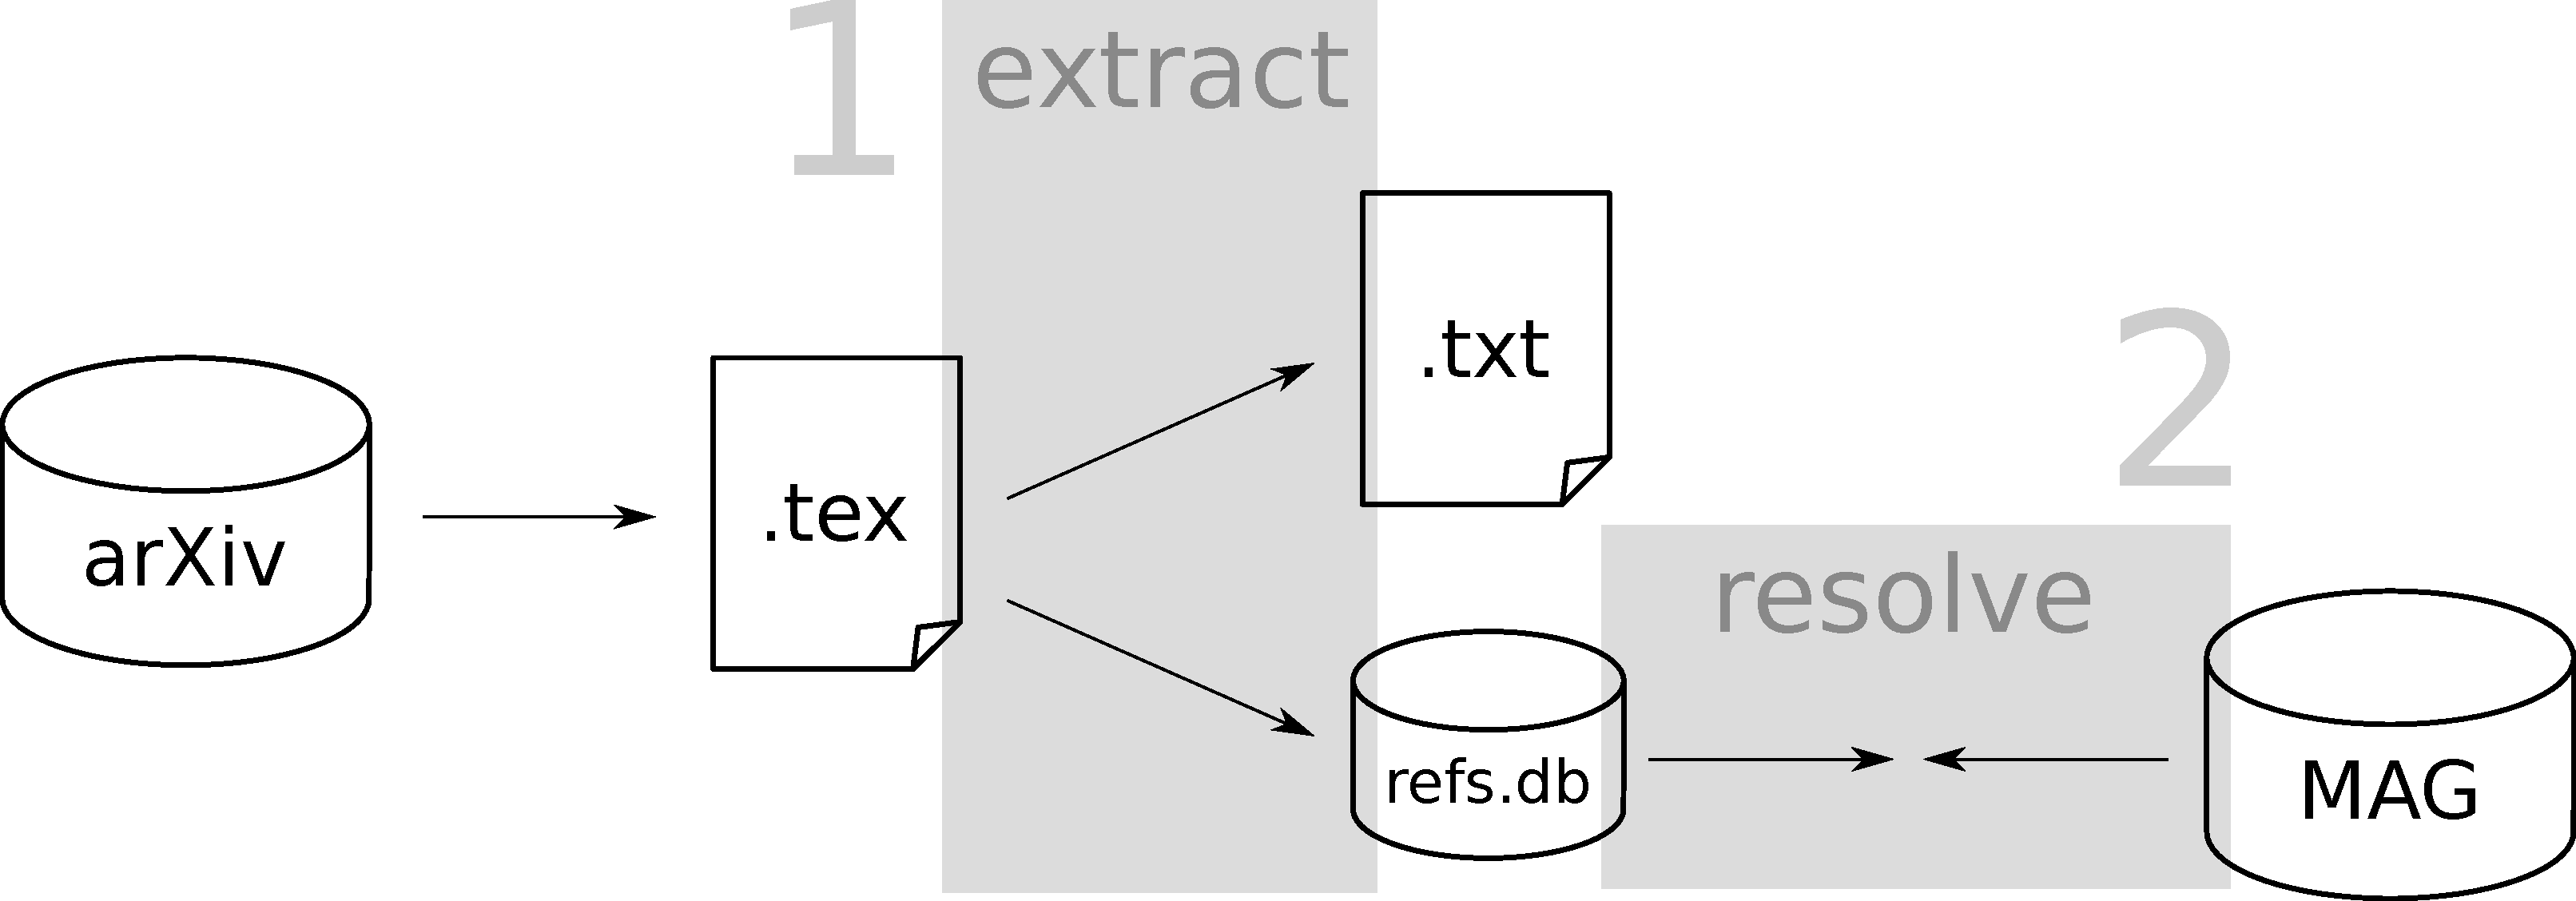
\includegraphics[width=.7\textwidth]{figures/corpus/Fig1.pdf}
  \caption{Schematic representation of the data set generation process}
  \label{fig:datagen}
\end{figure}

To create the data set, we start out with arXiv sources (see Fig.~\ref{fig:datagen}). From these we generate, per publication, a plain text file with the document's textual contents and a set of database entries reflecting the document's reference section. Association between reference strings and in-text citation locations are preserved by placing citation markers in the text. In a second step, we then iterate through all reference strings in the database and match them against paper metadata records in the MAG. This gives us full-text arXiv papers with (word level precision) citation links to MAG paper IDs. As a final step, we enrich the data with MAG IDs on the citing paper side (in addition to the already present arXiv IDs) and arXiv IDs on the cited paper side (in addition to the already present MAG IDs)---this is a straightforward process, because the paper metadata in the MAG includes source URLs, meaning papers found on arXiv have an arXiv.org source URL associated with them, such that a mapping from arXiv IDs to MAG IDs can be created.

Listing~\ref{lst:formatall} shows how our data set looks like. In the following, we describe the main steps of the data set creation process in more detail.

\subsection{\LaTeX{} Parsing}
In the following, we will describe the tools considered for parsing \LaTeX{}, the challenges we faced in general and with regard to arXiv sources in particular, and our resulting approach.

\subsubsection{Tools}

\begin{table}[tb]
\centering
  \caption{Comparison of tools for parsing \LaTeX{}}
  \label{tbl:tools}
\begin{small}
\begin{threeparttable}
\begin{tabular}{llll}
\toprule
    Tool & Output & Robust & Usable as is \\
   \midrule
    plastex\tnote{a} & DOM & no & yes\\
    TexSoup\tnote{b} & document tree & no & yes\\
    opendetex\tnote{c}\,/detex\tnote{d} & plain text & no & yes\\
    GrabCite~\cite{Faerber2018LREC} & plain\hphantom{ }text\hphantom{ }+ resolved ref. & yes & no\\
    LaTeXML\tnote{e} & XML & yes & yes\\
    Tralics\tnote{f} & XML & yes & yes\\
  \bottomrule
\end{tabular}  \begin{tablenotes}
    \item[a] See \refurlinline{https://github.com/tiarno/plastex}{2023-11-06}.
    \item[b] See \refurlinline{https://github.com/alvinwan/texsoup}{2023-11-06}.
    \item[c] See \refurlinline{https://github.com/pkubowicz/opendetex}{2023-11-06}.
    \item[d] See \refurlinline{https://www.freebsd.org/cgi/man.cgi?query=detex}{2023-11-06}.
    \item[e] See \refurlinline{https://github.com/brucemiller/LaTeXML}{2023-11-06}.
    \item[f] See \refurlinline{https://www-sop.inria.fr/marelle/tralics/}{2023-11-06}.
  \end{tablenotes}
\end{threeparttable}
\end{small}
\end{table}

We took several tools for a direct conversion from \LaTeX{} to plain text or to intermediate formats into consideration and evaluated them. Table \ref{tbl:tools} gives an overview of our results. Half of the tools failed to produce any output for a large amount of arXiv documents we used as test input and were therefore deemed not robust enough. \textit{GrabCite} \cite{Faerber2018LREC} is able to parse 78.5\%
of arXiv CS documents but integrates resolving references (see Sec.~\ref{sec:refresol}) against DBLP into the parsing process and therefore would require significant modification to fit our new system architecture. \textit{LaTeXML} and \textit{Tralics} are both robust and can be used as \LaTeX{} conversion tools as is. Based on subsequent tests, we observed that \textit{LaTeXML} needs on average 7.7 seconds (3.3 if formula environments are heuristically removed beforehand) to parse an arXiv paper, while \textit{Tralics} needs 0.09. Because the quality of their output seemed comparable, we chose to use \textit{Tralics}.

\subsubsection{Challenges}\label{sec:refresolchallenges}
Apart from the general difficulty of parsing \LaTeX{} due to its feature richness and people's free-spirited use of it, we especially note difficulty in dealing with extra packages not included in documents' sources.\footnote{The arXiv guidelines specifically suggest the omission of such (see \refurlinline{https://arxiv.org/help/submit_tex\#wegotem}{2023-11-06}).} While \textit{Tralics}, for example, is supposed to deal with \textit{natbib} citations,\refurl{https://www-sop.inria.fr/marelle/tralics/packages.html\#natbib}{2023-11-06} normalization of such citations leads to a decrease of citation markers not being able to be matched to an entry in the document's reference section from 30\% to 5\% in a sample of 565,613 citations we tested.

\subsubsection{Resulting Approach}
Our \LaTeX{} parsing solution consists of three steps: flattening, parsing, and output generation. First, we flatten each arXiv document's sources to a single \LaTeX{} file using \textit{latexpand}\refurl{https://ctan.org/pkg/latexpand}{2023-11-06}\textsuperscript{,}\footnote{We also tested flatex (\refurlinline{https://ctan.org/pkg/flatex}{2023-11-06}) and flap (\refurlinline{https://github.com/fchauvel/flap}{2023-11-06}) but got the best results with latexpand.} and normalize citation commands (e.g. \texttt{\textbackslash citep*}, \texttt{\textbackslash citet[see]}, \texttt{\textbackslash citealt}, etc. to \texttt{\textbackslash cite}) to prevent parsing problems later on. In the second step, we then generate an XML representation of the \LaTeX{} document using \textit{Tralics}. Lastly, we go through the generated XML structure and produce two types of output---(i)~an annotated plain text file with the document's textual contents and (ii)~database entries reflecting the document's reference section. For (i) we replace XML nodes that represent formulas, figures, tables, as well as intra-document references with replacement tokens and turn XML nodes originating from citation markers in the \LaTeX{} source (i.e., \texttt{\textbackslash cite}) into plain text citation annotation markers. For (ii), each entry in the document's reference section is assigned a unique identifier, its text is stored in a database, and the identifier put into the corresponding annotation in the plain text (cf. Listing~\ref{lst:formatall}).

\subsection{Reference Resolution}
\label{sec:refresol}
Resolving references to globally consistent identifiers (e.g. detecting that the reference strings (1), (2), and (3) in Listing~\ref{lst:refitems} all reference the same document) is a challenging and still unsolved task~\cite{Nasar2018}. Given it is the most distinctive singular part of a publication, we base our reference resolution on the title of the cited work and use other pieces of information (e.g., the authors' names) only in secondary steps. In the following, we will describe the challenges we faced, matching arXiv documents' reference strings against MAG paper records, and how we approached the task.

\subsubsection{Challenges}
Reference resolution can be challenging when reference strings contain only minimal amounts of information, when formulas or other special notation is used in titles, or when they refer to non publications (e.g., Listing~\ref{lst:refitems}, (4)--(6)).  Another problem we encountered was noise in the MAG. One such case are the MAG papers with IDs \texttt{2167727518} and \texttt{2763160969}. Both are identically titled \emph{``Observation of a new boson at a mass of 125 GeV with the CMS experiment at the LHC''} and dated to the year 2012. But while the former is cited 17k times and cites 112 papers within the MAG, the latter is a neither cited nor cites any other papers.\footnote{The MAG record with ID \texttt{2763160969} appears to be a noisy duplicate caused by a web source with easily misinterpretable author information (only a partial list is displayed).} Taking the number of citations into account when matching references, reduced the number of mismatches in this particular case from 2,918 to 0 and improved the overall quality of matches in general.

\begin{lstlisting}[caption={Examples of reference strings},label={lst:refitems}]
(1) V. N. Senoguz and Q. Shafi, arXiv:hep-ph/0412102
(2) V.N. Senoguz and Q. Shafi, Phys. Rev. D 71 (2005) 043514.
(3) V. N. Senoguz and Q. Shafi, ''Reheat temperature in supersymme
    tric hybrid inflation models,'' Phys. Rev. D 71, 043514 (2005)
     [hep-ph/0412102].
(4) V.Sauli, JHEP 02, 001 (2003).
(5) Aaij, Roel, et al. "Search for the $B^{0}_{s} \to \eta^{\prime
    }\phi$ decay" Journal of High Energy Physics 2017.5 (2017): 15
    8.
(6) According to the numerous discussions with my colleagues <remo
    ved> and <removed> an experimental verification of our theoret
    ical predictions is feasible.
\end{lstlisting}

\subsubsection{Resulting Approach}
Our reference resolution procedure can be broken down in two steps: title identification and matching. If contained in the reference string, title identification is performed based on an arXiv ID or DOI (where we retrieve the title from an arXiv metadata dump or via crossref.org\refurl{https://www.crossref.org/}{2023-11-06}); otherwise we use Neural ParsCit~\cite{Animesh2018}.\footnote{For title identification we also considered two other state of the art~\cite{Tkaczyk2018} tools, namely  CERMINE~\cite{Tkaczyk2015} and GROBID~\cite{Lopez2009}. However, we found CERMINE to be considerably slower than the other tools. And while GROBID showed comparable speed and output quality in preliminary tests, Neural ParsCit's tag based output format was more straightforward to integrate than the faceted TEI format structures that GROBID's reference parser module returns.}
The identified title is then matched against the normalized titles of all publications in the MAG. Resulting candidates are considered, if at least one of the author's names (as given in the MAG) is present in the reference string. If multiple candidates remain, we judge by the citation count given in the MAG---this particularly helps mitigate matches to rouge almost-duplicate entries in the MAG, which often have few to no citations, like paper \texttt{2763160969} mentioned in the previous section.

\subsection{Result format}
Listing \ref{lst:formatall} shows some example content from the data set. In addition to the paper plain text files and the references database, we also provide the citation contexts of all successfully resolved references extracted to a CSV file as well as a script to create custom exports.\footnote{See Python script \texttt{extract\_contexts.py} bundled with the data set for details.} For the provided CSV export, we set the citation context length to 3 sentences---the sentence containing the citation as well as the one before and after---as used by \cite{Tang2014fixed} and \cite{Huang2015fixed}. Each line in an export CSV has the following columns: cited MAG ID, adjacent cited MAG IDs, citing MAG ID, cited arXiv ID, adjacent cited arXiv IDs, citing arXiv ID, text (see bottom of Listing~\ref{lst:formatall}). Citations are deemed adjacent, if they are part of a citation group or are at most 5 characters apart (e.g. ``\emph{[27,42]''}, \emph{``[27], [42]''} or \emph{``[27] and [42]''}). The IDs of adjacent cited documents are added, because those documents are cited in an almost identical context (i.e. only a few characters to the left or right).
% Sentence tokenization for the extraction is performed with NLTK's pre-trained PunktSentenceTokenizer.

\begin{lstlisting}[caption={Excerpts from (top to bottom) a paper's plain text, corresponding entries in the references database, entries in the MAG, and extracted citation context CSV},label={lst:formatall}]
It has over 79 million images stored at the resolution of FORMULA 
. Each image is labeled with one of the 75,062 non-abstract nouns 
in English, as listed in the Wordnet{{cite:9ad20b7d-87d1-47f5-aeed
-10a1cf89a2e2}}{{cite: 298db7f5-9ebb-4e98-9ecf-0bdda28a42cb}} lexi
cal database.
------------------------------------------------------------------
[uuid]         [citing..] [cited..]   ...  [reference_string]
9ad20b7d-87d1  1412.3684  2081580037  ...  George A. Miller (1995)
-47f5-aeed-..                              . WordNet: A Lexical ..
298db7f5-9ebb  1412.3684  2038721957  ...  Christiane Fellbaum (19
-4e98-9ecf-..                              98), ""WordNet: An El..
------------------------------------------------------------------
[paperid]   [originaltitle]                           [publ..]  ..
2038721957  WordNet : an electronic lexical database  MIT Press ..
2081580037  WordNet: a lexical database for English   ACM       ..
------------------------------------------------------------------
2131463865|2038721957|2081580037|1412.3684|||It has over 79 millio
n images stored at the resolution of FORMULA . Each image is label
ed with one of the 75,062 non-abstract nouns in English, as listed
 in the Wordnet CIT MAINCIT lexical database. It has been noted th
at many of the labels are not reliable CIT .
\end{lstlisting}

\section{Statistics and Key Figures}
\label{sec:statistics}

In this section we present the data set and its creation process in terms of numbers. Furthermore, insight into the distribution of references and citation contexts is given.

\subsection{Creation Process}
We used an arXiv source dump containing all documents up until the end of 2018 (1,492,923 documents). 114,827 of these were only available in PDF format, leaving 1,378,096 sources. Our pipeline output 1,283,584 (93.1\%) plain text files, 1,139,790 (82.7\%) of which contained citation markers. The number of reference strings identified is 39,694,083, for which 63,633,427 citation markers were placed within the plain text files. This first part of the process took 67 hours to run, unparallelized on a 8 core Intel Core i7-7700 3.60GHz machine with 64 GB of memory.

Of the 39,694,083 reference strings, we were able to match 16,926,159 (42.64\%) to MAG paper records. For 31.32\% of the reference strings we could neither find an arXiv ID or DOI, nor was Neural ParsCit able to identify a title.\footnote{To assess whether or not the large percentage of reference strings without identified title is due to Neural ParsCit missing a lot of them, we manually check its output for a random sample of 100 papers (4027 reference strings). We find that 99\% of cases with no title identified actually do not contain a title---like for example items (1), (2) and (4) in Lst.~\ref{lst:refitems}. These kind of references seem to be most common in physics papers. The 1\% where a title was missed were largely references to non-English titles and books. We therefore conclude that the observed numbers largely reflect the actual state of reference strings rather than problems with the approach taken.} For the remaining 26.04\% a title was identified, but could not be matched to the MAG.
Of the matched 16.9 million items' titles, 52.60\% were identified via Neural ParsCit, 28.31\% by DOI and 19.09\% by arXiv ID. Of the identified DOIs, 32.9\% were found as is, while 67.1\% were heuristically determined. This was possible because the DOIs of articles in journals of the American Physical Society follow predictable patterns. The matching process took 119 hours, run in 10 parallel processes on a 64 core Intel Xeon Gold 6130 2.10GHz machine with 500 GB of memory.

Comparing the performance of our approach using all papers (1991--2018) to using only the papers from 2018 (i.e. recent content), we note that the percentage of successfully extracted plain texts goes up from 93.1 to 95.9\% (82.7 to 87.8\% only counting plain text files containing citation markers) and the percentage of successfully resolved references increases from 42.64 to 59.39\%. A possible explanation for the latter would be, that there is more and higher quality metadata coverage (MAG, crossref.org, etc.) of more recent publications.

\begin{figure}[!ht]
  \centering
  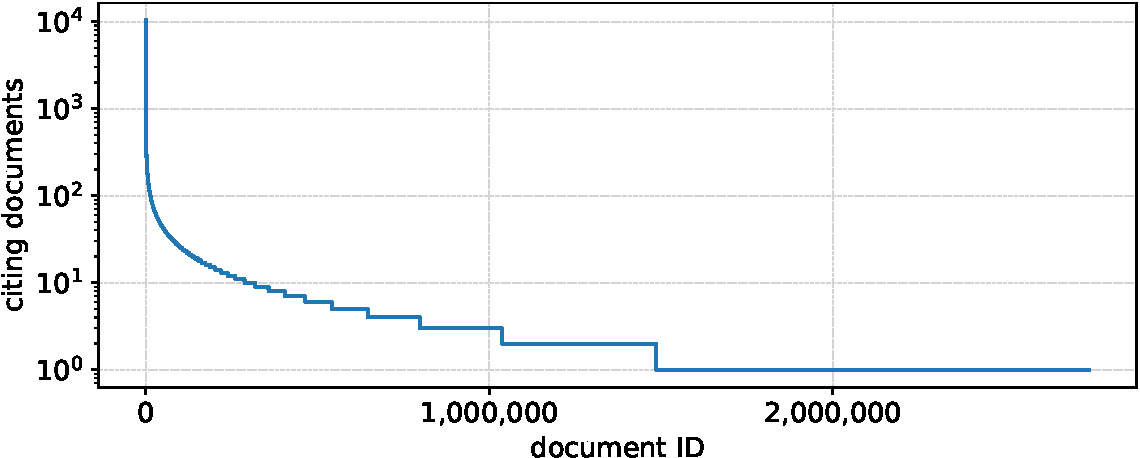
\includegraphics[width=0.92\linewidth]{figures/corpus/Fig2.pdf}
  \caption{Number of citing documents per cited document}
  \label{fig:numcitdoc}
  \vspace{1em}
%\end{figure}
%\begin{figure}[ht]
%  \centering
  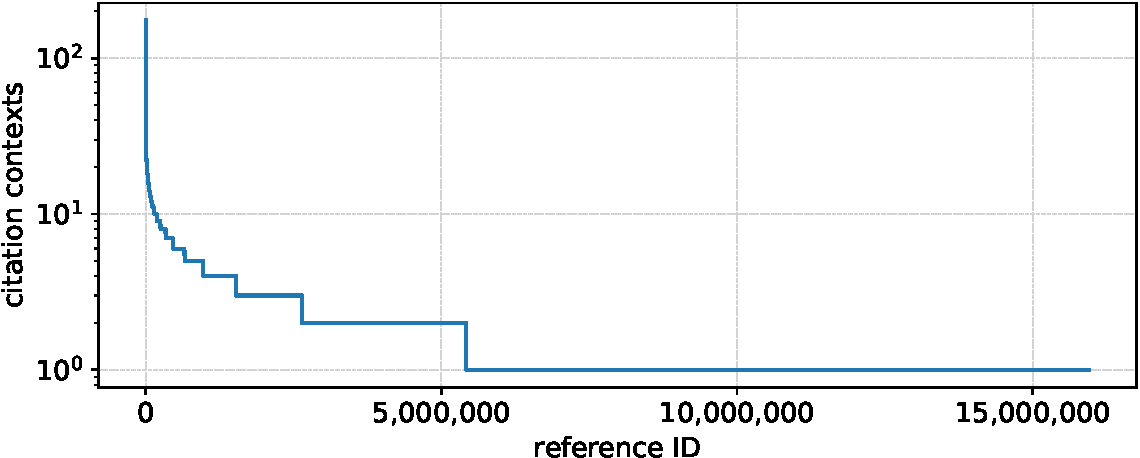
\includegraphics[width=0.92\linewidth]{figures/corpus/Fig3.pdf}
  \caption{Number of citation contexts per reference}
  \label{fig:numcontref}
    \vspace{1em}
\end{figure}

\subsection{Resulting Data Set}
Our data set consists of \emph{2,746,288 cited papers, 1,043,126 citing papers, 15,954,664 references and 29,203,190 citation contexts}.\footnote{References that were successfully matched to a MAG record but have no associated citation markers (due to parsing errors; cf. Sec.~\ref{sec:refresolchallenges}) are not counted here.} 
% DB entry figures (not excluding cases where no marker is present):
% cited: 2,820,381
% citing: 1,192,097
% references: 16,802,498

\begin{figure}[tb]
  \centering
    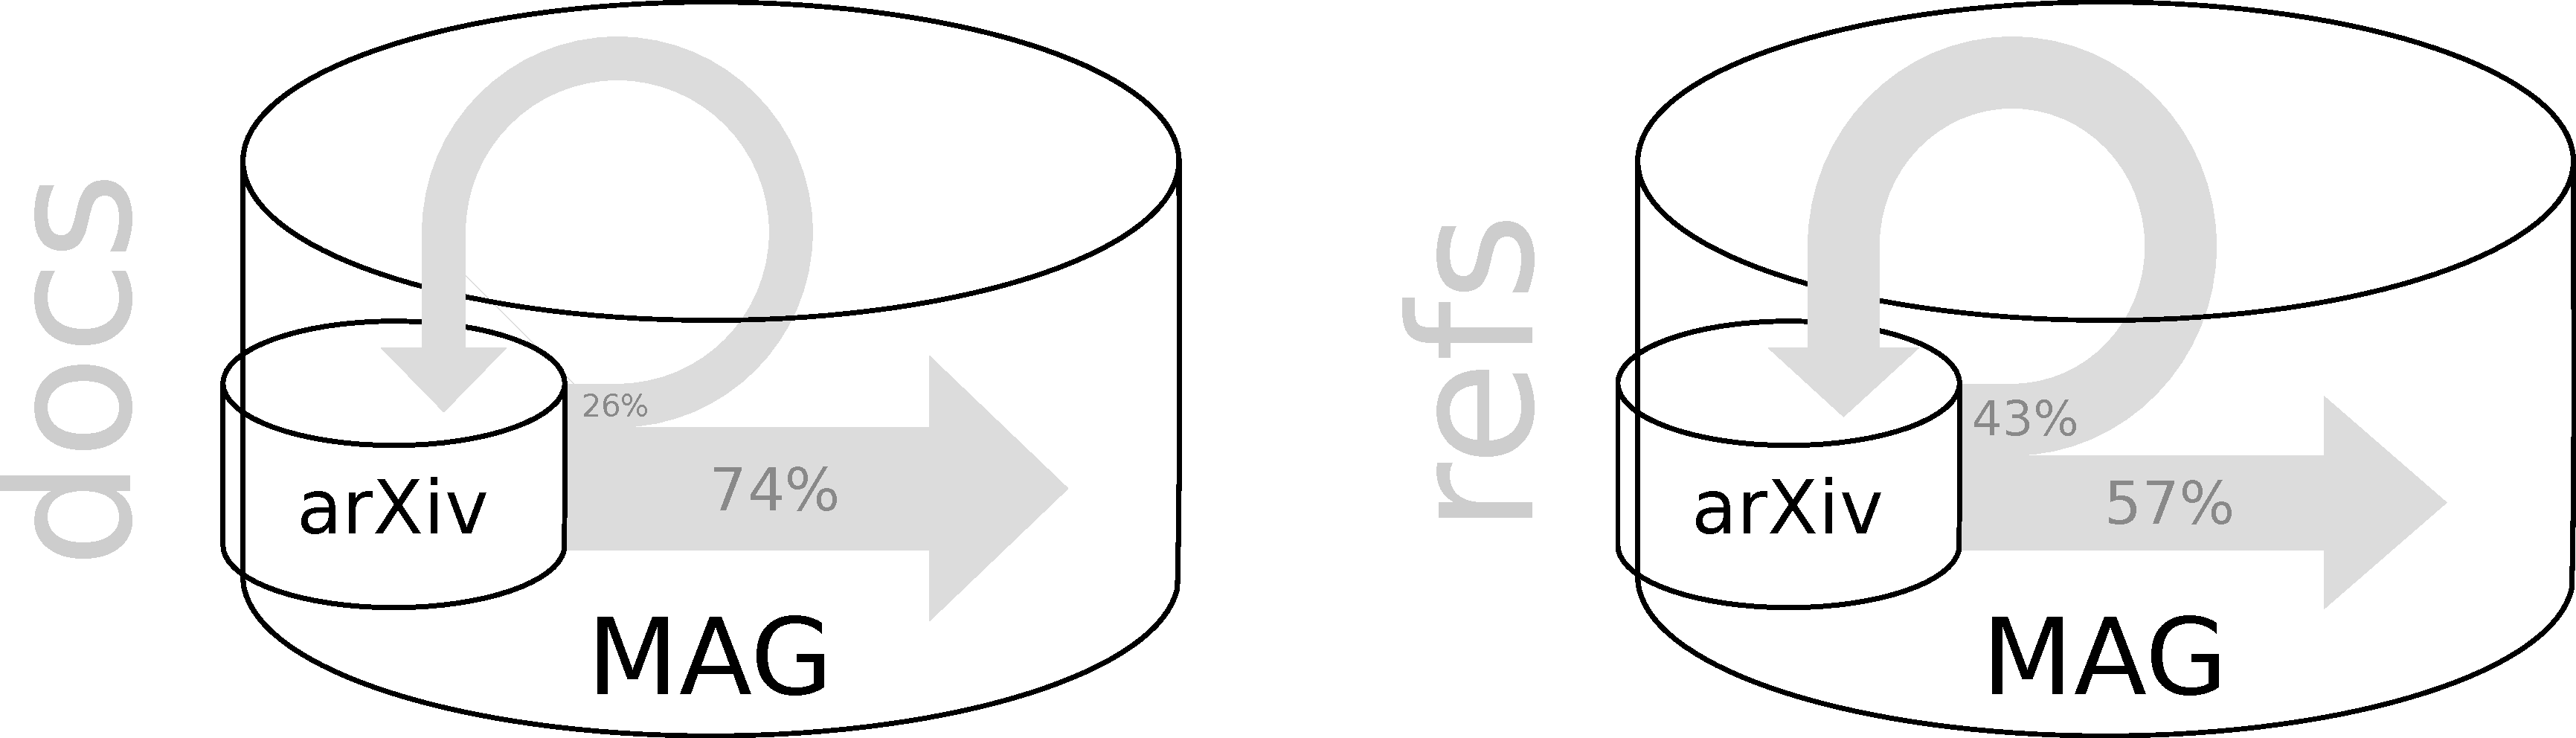
\includegraphics[width=.9\textwidth]{figures/corpus/Fig4.pdf}
  \caption{Visualization of the citation flow in terms of documents and references from arXiv to the MAG}
  \label{fig:inflow}
\end{figure}

Figure \ref{fig:numcitdoc} shows the number of citing documents for all cited documents. There is one cited document with over 10,000 citing documents, another 8 with more than 5,000 and another 14 with more than 3,000. 1,485,074 (54.07\%) of the cited documents are cited at least two times, 646,509 (23.54\%) at least five times. The mean number of citing documents per cited document is 5.81 (SD 28.51). Figure \ref{fig:numcontref} shows the number of citation contexts per entry in a document's reference section. 10,537,235 (66.04\%) entries have only one citation context, the maximum is 278, the mean 1.83 (SD 2.00).

Because not all documents referenced by arXiv papers are hosted on arXiv itself, we additionally visualize the citation flow with respect to the MAG in Figure \ref{fig:inflow}. 95\% of our citing documents are contained in the MAG. Of the cited documents, 26\% are contained in arXiv and therefore included as full-text, while 74\% are only included as MAG IDs. On the level of references, this distribution shifts to 43/57. The high percentages of citation links contained within the data set can be explained due to the fact, that in physics and mathematics---which make up a large part of the data set---it is common to self-archive papers on arXiv.

\section{Evaluation of Citation Data Validity and Coverage}
\label{sec:evaluation-validity-and-coverage}

\subsection{Citation Data Validity}
\label{sec:evaluation-reference-resolution}
To evaluate the validity of our reference resolution results, we take a random sample of 300 matched reference strings and manually check for each of them, if the correct record in the MAG was identified. This is done by viewing the reference string next to the matched MAG record and verifying, if the former actually refers to the latter.\footnote{Further details can be found at \refurlinline{https://github.com/IllDepence/unarXive/tree/legacy_2020/doc/matching_evaluation}{2023-11-06}.} Given the 300 items, we observed 3 errors, giving us an accuracy estimate of 96\% at the worst, as shown in Table~\ref{tbl:confvals}. Table~\ref{tbl:mismatches} shows the three incorrectly identified documents. In all three cases the misidentified document's title is contained in the correct document's title, and there is a large or complete author overlap between correct and actual match. This shows that authors sometimes title follow-up work very similarly, which leads to hard to distinguish cases.

\begin{table}[tb]
  \caption[Confidence intervals for a sample size of 300]{Confidence intervals for a sample size of 300 with 297 positive results as given by Wilson score interval and Jeffreys interval \cite{Brown2001}}
  \label{tbl:confvals}
  \centering
  \begin{small}
\begin{tabular}{c@{\hspace{0.1in}}c@{\hspace{0.1in}}c@{\hspace{0.1in}}c}
\toprule
    Confidence level & Method & Lower limit & Upper limit \\
\midrule
    0.99 & Wilson & 0.9613 & 0.9975 \\\noalign{\smallskip}
    \ & Jeffreys & 0.9666 & 0.9983 \\\noalign{\smallskip}
    \hline\noalign{\smallskip}
    0.95 & Wilson & 0.9710 & 0.9966 \\\noalign{\smallskip}
    \ & Jeffreys & 0.9736 & 0.9972 \\
    \bottomrule
\end{tabular} 
\end{small}
\end{table}

\begin{table}[tb]
  \caption{Mismatched documents}
  \label{tbl:mismatches}
  \centering
  \begin{small}
\begin{tabular}{c@{\hspace{0.1in}}l@{\hspace{0.1in}}m{10cm}}
\toprule
    \# & \  & Document \\
\midrule
    1 & matched & \emph{``The Maunder Minimum''} (John A. Eddy; 1976) \\\noalign{\smallskip}
    \ & correct & \emph{``The Maunder Minimum: A reappraisal''} (John A. Eddy; 1983) \\\noalign{\smallskip}
    \hline\noalign{\smallskip}
    2 & matched & \emph{``Support Vector Machines''} (Gareth James, Daniela Witten, Trevor Hastie, Robert Tibshirani; 2013) \\\noalign{\smallskip}
    \ & correct & \emph{``1-norm Support Vector Machines''} (Ji Zhu, Saharon Rosset, Robert Tibshirani, Trevor J. Hastie; 2003) \\\noalign{\smallskip}
    \hline\noalign{\smallskip}
    3 & matched & \emph{``The Putative Liquid-Liquid Transition is a Liquid-Solid Transition in Atomistic Models of Water''} (David Chandler, David Limmer; 2013) \\\noalign{\smallskip}
    \ & correct & \emph{``The putative liquid-liquid transition is a liquid-solid transition in atomistic models of water. II''} (David T. Limmer, David Chandler; 2011) \\\noalign{\smallskip}
    \bottomrule
\end{tabular} 
\end{small}
\end{table}

\subsection{Citation Data Coverage}
For the 95\% of our data set, where citing as well as cited document have a MAG ID, we are able to compare our citation data directly to the MAG. The composition of reference section coverage (i.e. how many of the references are reflected in each of the data sets) of all 994,351 citing documents can be seen in Figure \ref{fig:citcomp}.  Of the combined 26,205,834 reference links, 9,829,797 are contained in both data sets (orange), 5,918,128 are in unarXive only (blue), and 10,457,909 are in the MAG only (green). On the document level we observe, that for 401,046 documents unarXive contains more references than the MAG, and for 545,048 it is the other way around. The striking difference between reference and document level\footnote{While the number of reference links exclusive to the MAG is about twice as high as the number of reference links exclusive to unarXive, the number of documents for which either of the data sets has better coverage is on a comparable level.} suggests, that the MAG has better coverage of large reference sections. This is supported by the fact that citing papers, where the MAG contains more references, cite on average 34.28 documents, while the same average for citing papers, where unarXive contains more references, is 17.46. Investigating further, in Figure \ref{fig:citcount2balance} we look at the number of citing documents in terms of reference section \emph{size} (x-axis) and \emph{exclusive coverage in unarXive and MAG}\footnote{Calculated as $\frac{\text{\#citations only in unarXive }-\text{ \#citations only in MAG}}{\text{\#citations in both }+\text{ \#citations only in unarXive }+\text{ \#citations only in MAG}}$.} (y-axis). As we can see (and as the almost exclusively blue area on the right hand side of Figure \ref{fig:citcomp} suggests), there is a large number of papers, citing $\leq 50$ documents, where $\geq 80\%$ of the reference section are only contained in unarXive. Put differently, there is a large portion of documents, where the reference section is covered to some degree by unarXive, but has close to no coverage in the MAG. The number of citing documents, where the MAG contains $0$ references whereas unarXive has $\ge 1$, is 215,291---these have an average of 15.1 references in unarXive.\footnote{Manually looking into a sample of 100 of these documents, we find the most salient commonality to be irregularities w.r.t. to the reference section headline. 58 of the papers (55 physics, 2 quantitative biology, 1 CS) have no reference section headline, 2 have a double reference section headline and further 2 have the headline directly followed by a page break. The reason for the large number of MAG documents with no references might therefore be, that the PDF parser used can not yet deal with such cases.} The number of citing documents (within the 994,351 at hand), where unarXive contains $0$ references whereas the MAG has $\ge 1$, is 0.

\begin{figure}[tb]
  \centering
    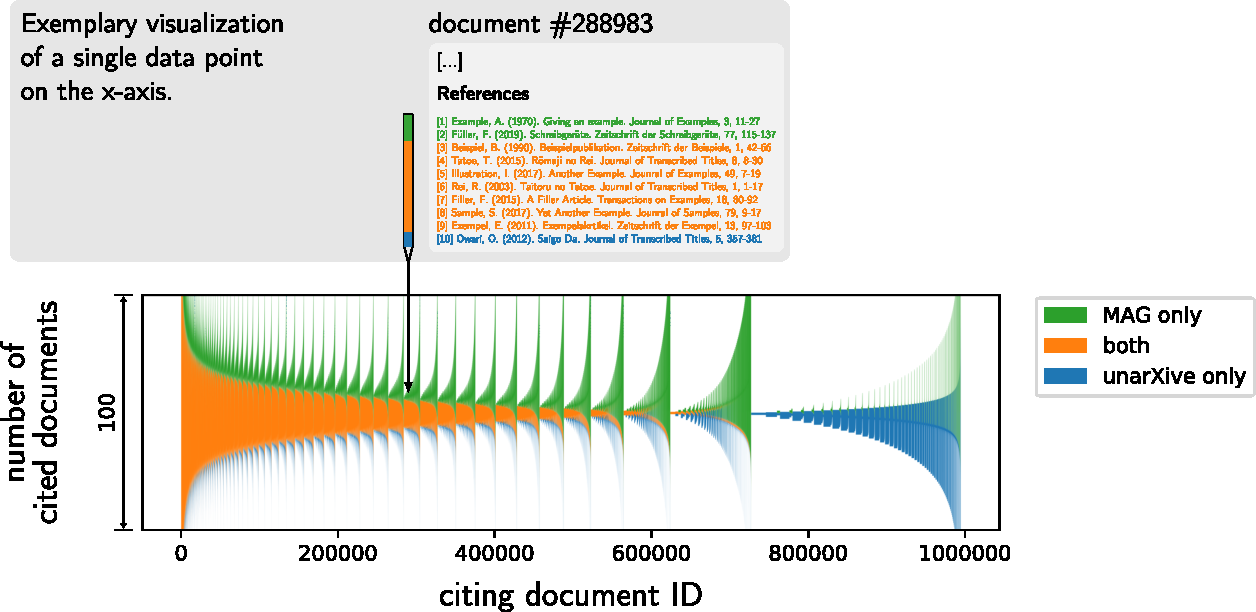
\includegraphics[width=\textwidth]{figures/corpus/Fig5.pdf}
  \caption[Composition of reference section coverage for all citing documents]{Composition of reference section coverage for all citing documents (cut off at 100 cited documents)}
  \label{fig:citcomp}
\end{figure}

\begin{figure}[tb]
  \centering
    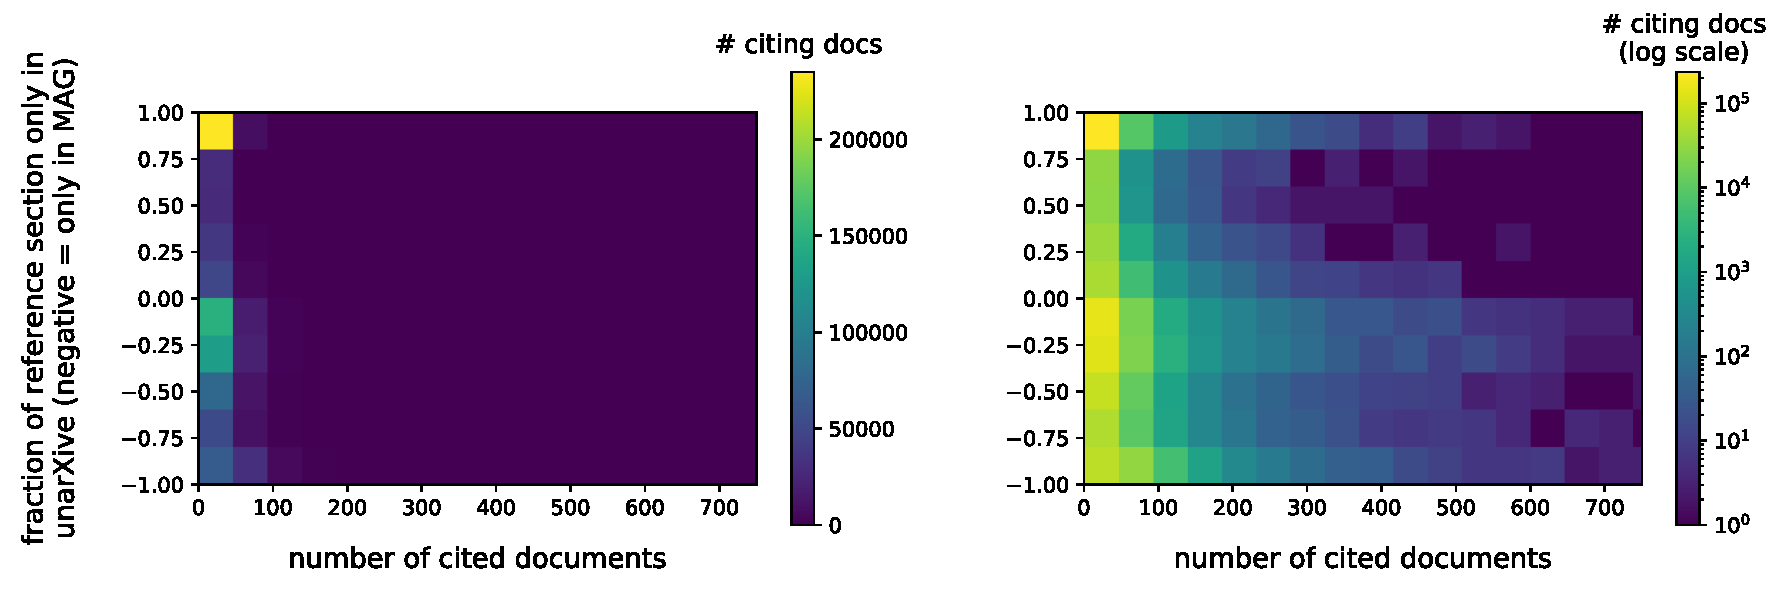
\includegraphics[width=\textwidth]{figures/corpus/Fig6.pdf}
  \caption[Distribution of citing documents in terms of reference section size and their coverage in unarXive and MAG]{Distribution of citing documents in terms of reference section size and their coverage in unarXive and MAG (cut off at 750 cited documents)}
  \label{fig:citcount2balance}
\end{figure}

Needless to say, additional references are only of value if they are valid. From both the citation links only found in unarXive, as well as those only found in the MAG, we therefore take a sample of 150 citing paper cited paper pairs and manually verify, if the former actually references the latter. This is done by inspecting the citing paper's PDF and checking the entries in the reference section against the cited paper's MAG record.\footnote{Further details can be found at \refurlinline{https://github.com/IllDepence/unarXive/tree/legacy_2020/doc/coverage_evaluation}{2023-11-06}.} On the unarXive side, we observe 4 invalid links, all of which are cases similar to those showcased in Table \ref{tbl:mismatches}. On the MAG side, we observe 8 invalid links. Some of them seem to originate from the same challenges as the ones we face, e.g. similarly titled publications by same authors, leading to misidentified \emph{cited} papers. Other error sources are, for instance, an invalid source for a \emph{citing} paper being used and its reference section parsed (e.g. paper ID \texttt{1504647293}, where one of the PDF sources is the third author's Ph.D. thesis instead of the described paper). Given that the citation links exclusive to unarXive appear to be half as noisy as those exclusive to the  MAG, we argue that the 5,918,128 links only found in unarXive could be useful for citation and paper based tasks using MAG data. This would especially be the case for the field of physics, as it makes up a significant portion of our data set.

\section{Analysis of Citation Flow and Citation Contexts}
\label{sec:analysis}

Because the documents in unarXive span multiple scientific disciplines, interdisciplinary analyses, such as the calculation of the flow of citations between disciplines, can be performed. Furthermore, the fact that documents are included as full-text and citation markers within the text are linked to their respective cited documents, makes varied and fine grained study of citation contexts possible. To give further insight into our data set, we therefore conduct several such analyses in the following. Note that, for interdisciplinary investigations, disciplines other than physics, mathematics, and computer science are combined into \emph{other} for space and legibility reasons, as they are only represented by a small number of publications. On the citing documents' side, these span the fields of economics, electrical engineering and systems science, quantitative biology, quantitative finance, and statistics. Combined on the cited documents' side are chemistry, biology, engineering, materials science, economics, geology, psychology, medicine, business, geography, sociology, political science, philosophy, environmental science, and art.

\subsection{Citation Flow}

\begin{figure}
  \centering
    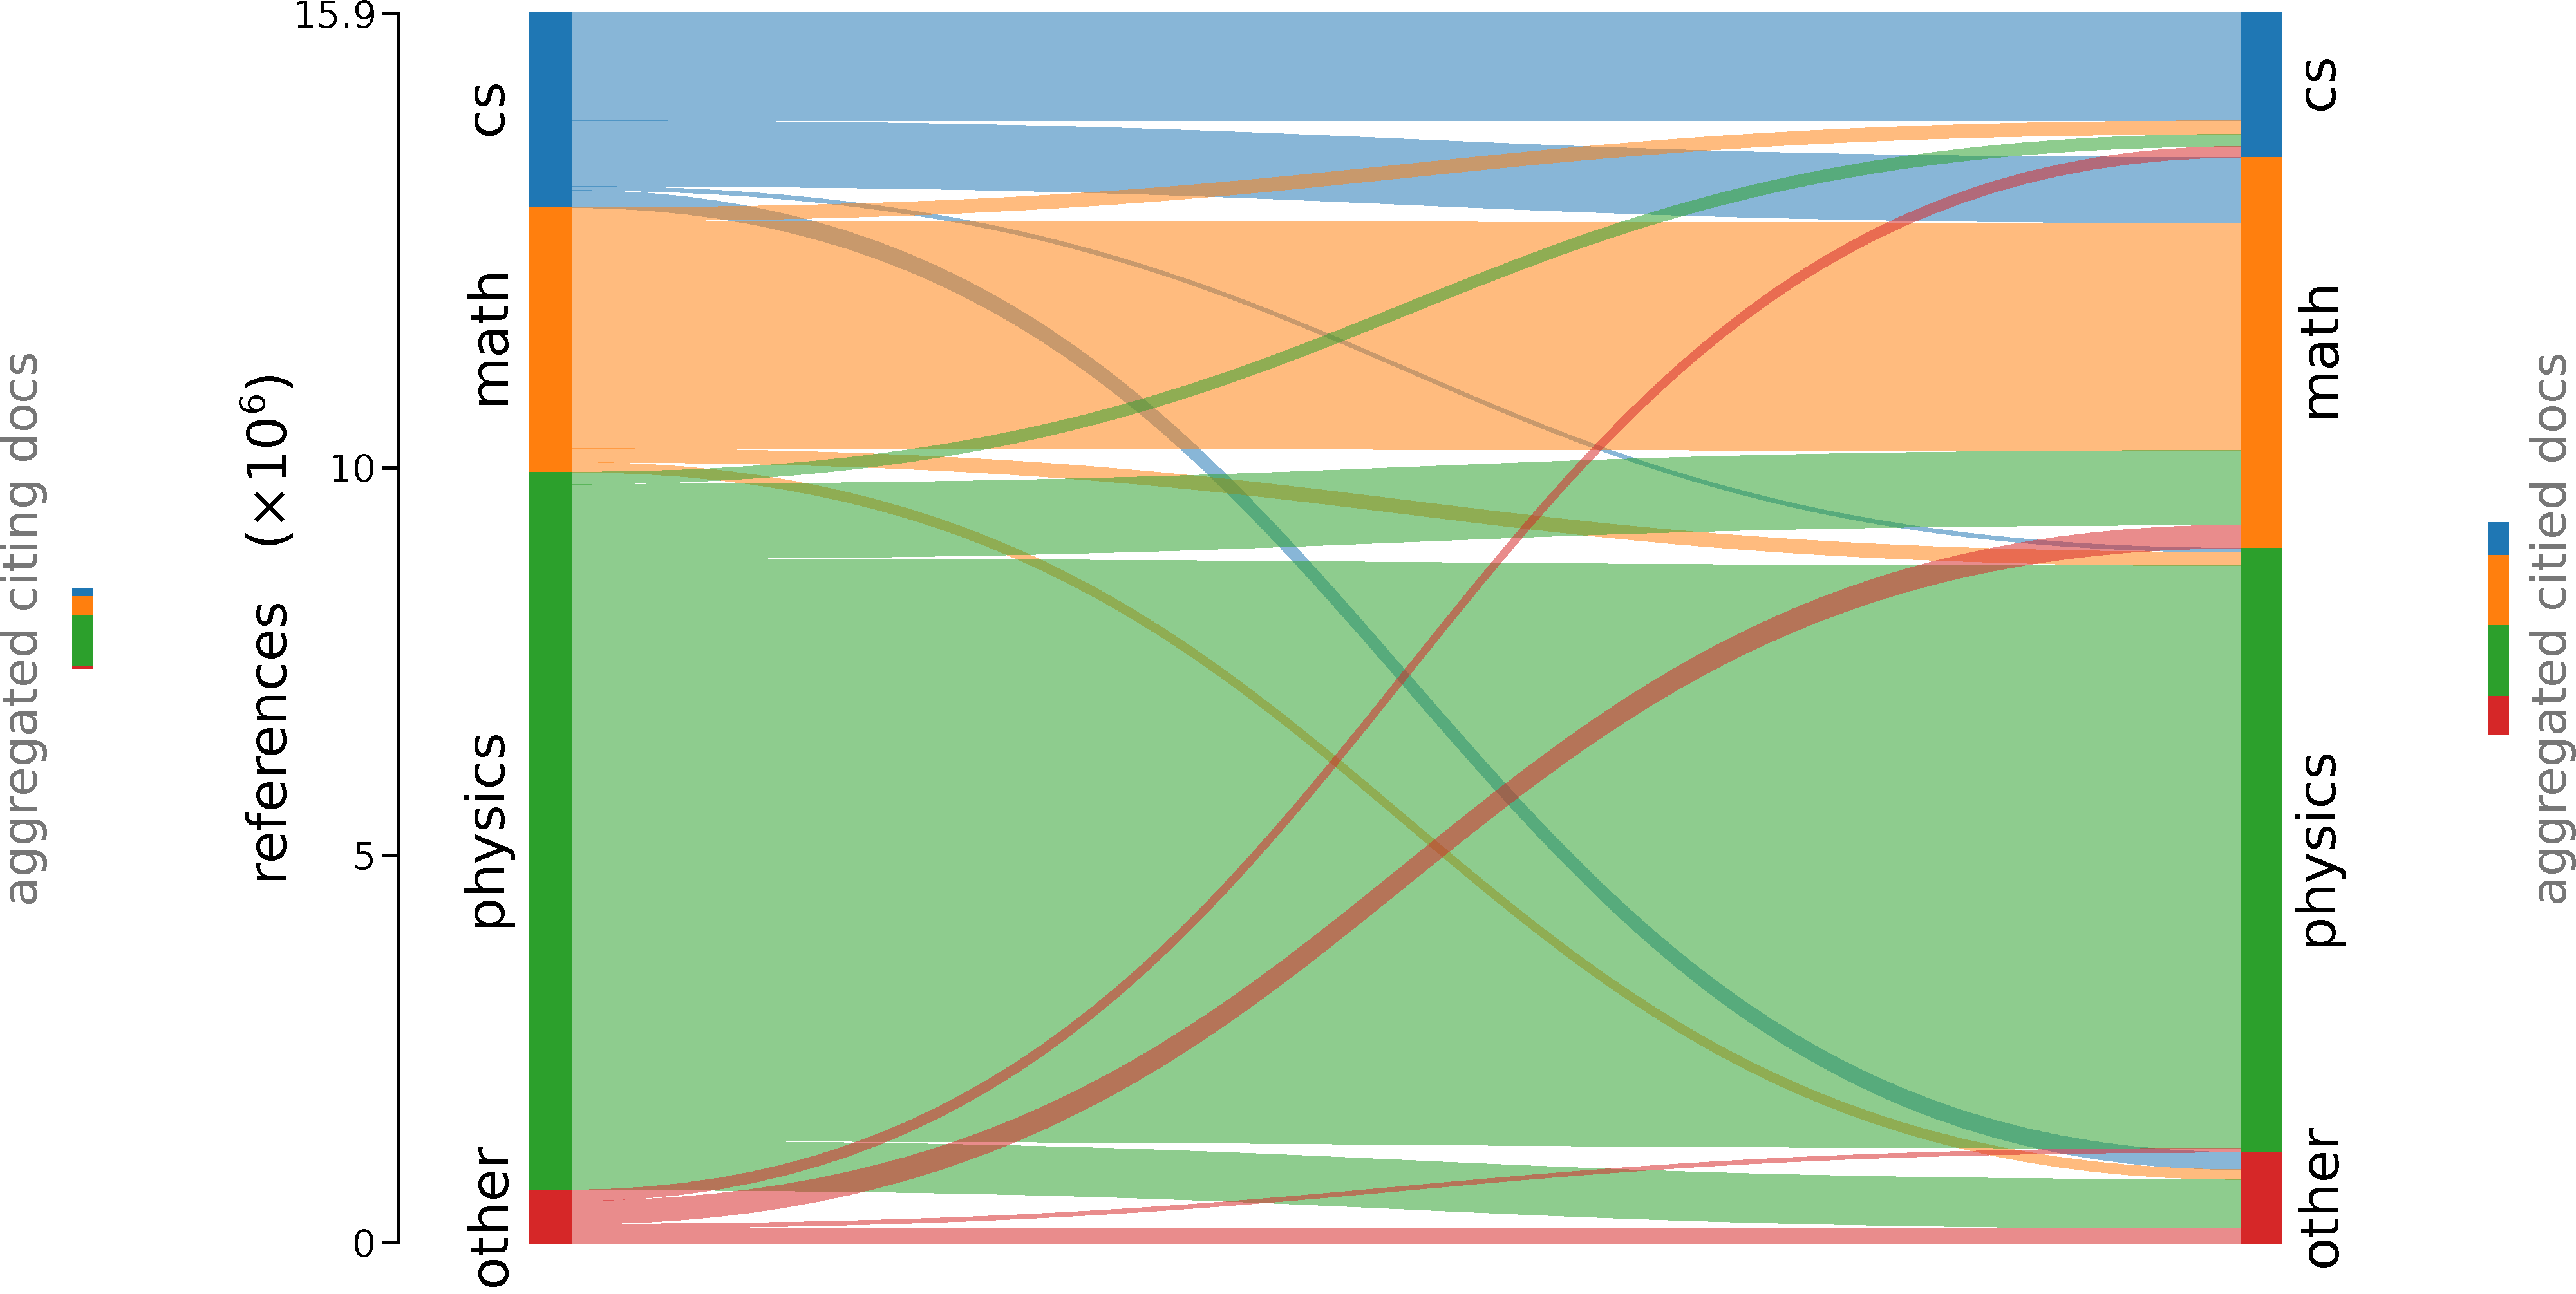
\includegraphics[width=0.97\textwidth]{figures/corpus/Fig7.pdf}
  \caption[Citation flow by discipline for 15.9 million references]{Citation flow by discipline for 15.9 million references (the number of citing and cited documents per discipline are plotted on the sides)}
  \label{fig:sankey}
\end{figure}

Figure \ref{fig:sankey} depicts the flow of citations by discipline for all 15.9 million matched references. As one would expect, publications in each field are cited the most from within the field itself. Notable is, that the incoming citations in mathematics are the most varied (physics and computer science combined make up 35\% of the citations). As citation contexts are useful descriptive surrogates of the documents they refer to \cite{Elkiss2008fixed}, a composition as varied as mathematics in Figure \ref{fig:sankey} bears the question as to whether a distinction by discipline could be worth considering, when using citation contexts as descriptions of cited documents. That is, computer scientists and physicists might refer to math papers in a different way than mathematicians do. Borders between disciplines are, however, not necessarily clear cut, meaning that such a distinction might not be as straight forward as the color coding in Figure \ref{fig:sankey} suggests.

\subsection{Availability of Citation Contexts}

\begin{figure}
  \centering
    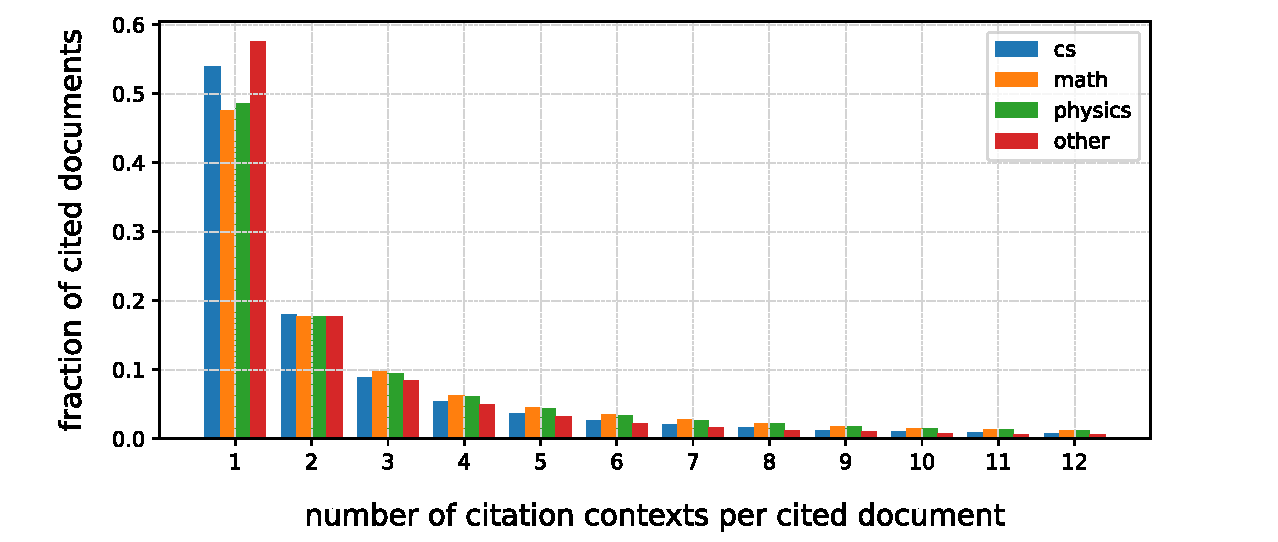
\includegraphics[width=\textwidth]{figures/corpus/Fig8.pdf}
  \caption{Normalized distribution of the number of citation contexts per cited document}
  \label{fig:citcontextdist}
\end{figure}

Another aspect that becomes relevant, when using citation contexts to describe cited documents, is the number of citation contexts available per cited publication. Figure \ref{fig:citcontextdist} shows, that the distribution of the number of citation contexts per cited document is similar across disciplines. In each discipline, around half of the cited documents are just mentioned once across all citing documents, 17.5\% exactly twice, and so on. The tail of the distribution drops a bit slower for physics and mathematics. The mean values of citation contexts per cited document are 9.5 (SD 50.3) in physics, 7.0 (SD 28.8) in mathematics, 5.1 (SD 31.1) in computer science and 3.5 (SD 11.0) for the combined other fields. This leads to two conclusions. First, it suggests that a representation relying solely on citation contexts may only be viable for a small fraction of publications. Second, the high dispersion in the number of available citation contexts shows that means might not be very informative when it comes to citation counts aggregated over specific sets of documents.

\subsection{Characteristics of Citation Contexts}
For our analysis of the contents of citation contexts, we focus on three aspects: whether or not citations are (1)~integral, (2)~syntactic and (3)~target section specific. These aspects were chosen, because they give particular insights into the citing behavior of researchers, as explained alongside the following definition of terms.

\subsubsection{``Integral'', ``Syntactic'' and ``Target Section Specific'' Citations}\label{sec:termdefs}
We first discuss the terms \emph{``integral''} and \emph{``syntactic''}, which are both established in existing literature. An integral citation is one, where the name of the cited document's author appears within the citing sentence \emph{and} has a grammatical role~\cite{Swales1990,Hyland1999} (e.g. ``Swales [73] has argued that ...''). Similarly, a citation is syntactic, if the \emph{citation marker} has has a grammatical role within the citing sentence~\cite{Whidby2011,Abujbara2012} (e.g. ``According to [73] it is ...''). Integral citations are seen as an indication of emphasis towards the cited author (where the opposite direction would be towards the cited work)~\cite{Swales1990,Hyland1999}. Syntactic citations are of interest, when determining how a citation relates to different parts of the citing sentence~\cite{Whidby2011,Abujbara2012}. Both qualities are relevant when studying the role of citations~\cite{Faerber2019TPDL}.

\begin{table}
\centering
    \caption[Examples of citations and their categorization into integral/non-\allowbreak integral as well as syntactic/non-syntactic]{Examples of citations and their categorization into integral/non-\allowbreak integral as well as syntactic/non-syntactic (``\checkmark''=yes, ``$\times$''=no, ``?''=unclear)}
    \label{tab:integralsyntactic}
\begin{center}
    \begin{tabular}{llll|ll}
    \toprule
    \ & \rotatebox{90}{\cite{Swales1990}} & \rotatebox{90}{\cite{Hyland1999}} & \rotatebox{90}{\cite{Lamers2018}} & \rotatebox{90}{\cite{Whidby2011}} & \rotatebox{90}{\cite{Abujbara2012}} \\
    \ & \ & \ & \ & \ & \ \\
    Context excerpt (citation marker {\color{UniBlue}highlighted}) & \multicolumn{3}{c|}{\textbf{integral}} & \multicolumn{2}{l}{\textbf{syntactic}} \\
    \midrule
    ``Swales {\color{UniBlue}(1990)} has argued that ...''                 & \checkmark & \checkmark & \checkmark & $\times$ & ? \\
    ``{\color{UniBlue}Swales (1990)} has argued that ...''                 & \checkmark & \checkmark & $\times$ & \checkmark & \checkmark \\
    ``Swales {\color{UniBlue}[73]} has argued that ...''                   & \checkmark & \checkmark & \checkmark & $\times$ & $\times$ \\
    ``Swales has argued that ... {\color{UniBlue}[73]}''                   & \checkmark & \checkmark & \checkmark & $\times$ & $\times$ \\
    ``It has been argued {\color{UniBlue}(Swales, 1990)} that ...''        & $\times$ & $\times$ & $\times$ & $\times$ & $\times$ \\
    ``It has been argued {\color{UniBlue}[73]} that ...''                  & $\times$ & $\times$ & $\times$ & $\times$ & $\times$ \\
    ``According to {\color{UniBlue}(Swales, 1990)} it is ...''             & ? & ? & $\times$ & \checkmark & \checkmark \\
    ``According to {\color{UniBlue}[73]} it is ...''                       & $\times$ & $\times$ & $\times$ & \checkmark & \checkmark \\
    ``... has been shown (see {\color{UniBlue}(Swales, 1990)}).''          & $\times$ & $\times$ & $\times$ & \checkmark & $\times$ \\
    \bottomrule
    \end{tabular}
\end{center}
\end{table}

Table~\ref{tab:integralsyntactic} gives a more detailed account of both terms' use in literature. Note that \cite{Lamers2018} provide a classification algorithm for integral and non-integral citations that slightly differs from Swales' original definition depending on the interpretation of a citation marker's scope, but also gives a clear classification in an edge case where Swales' definition is unclear. Furthermore note, that the two ways for distinguishing syntactic and non-syntactic citations found in literature are not identical. This is in part because the method given by \cite{Abujbara2012} is kept rather simple. For the intents and purposes of our analysis we follow the definitions of Lamers et al. and Whidby et al. for \emph{``integral''} and \emph{``syntactic''} respectively.

\begin{table}
\centering
    \caption{Examples of target section specific citations}
    \label{tab:secspec}
\begin{center}
    \begin{tabular}{l}
    \toprule
    Context excerpt ({\color{UniBlue}concerns citing document} / {\color{RandomRed}concerns cited document}) \\
    \midrule
    ``See [73], {\color{RandomRed}Section 3}.'' \\
    ``This improves {\color{RandomRed}Lemma 2} of [73], which is ...'' \\
    ``Due to this, the proof is now similar to that of {\color{RandomRed}Theorem 6.4} from [73].'' \\
    ``The copolymer version of {\color{UniBlue}Theorem 7} was derived in [73], {\color{RandomRed}Theorem 3.2}.''  \\
    ``{\color{UniBlue}Figure 1} is qualitatively similar to {\color{RandomRed}Figure 3} in [73].'' \\
    \bottomrule
    \end{tabular}
\end{center}
\end{table}

As a third aspect for analysis, we define \emph{``target section specific''} citations as those citations, where a specific section within the citation's target (i.e. the cited document) is referred to. Examples are given in Table~\ref{tab:secspec}. Target section specific citations are of interest for two reasons. First, in a similar fashion to integral citations, they are a particular form of citing behavior that might be used to infer characteristics of the relationship between citing author and cited document (e.g. a focus on the document rather than authors, or in depth engagement or familiarity with the cited document's contents). Second, when using citation contexts as descriptions of cited documents, such as in citation context-based document summarization, target section specific citations might benefit from special handling, as their contexts only describe a (sometimes very narrow) part of the cited document.

In the following we will analyze all three aspects (integral, syntactic, target section specific) with respect to the different scientific disciplines covered by our data set.

\subsubsection{Manual Analysis of Citation Contexts}

\begin{table}[tb]
\centering
  \caption[Per discipline number of citations labeled integral, syntactic, imultaneously integral and syntactic, target section specific]{Per discipline number of citations labeled (1)~integral, (2)~syntactic, (3)~simultaneously integral and syntactic, (4)~target section specific (sample size = 300)}
  \label{tbl:integralsyntacticsecspec}
\begin{small}
\begin{tabular}{lrrrr}
\toprule
   Discipline & Integral & Syntactic & Integral+Syntactic & Target Section Specific \\
   \midrule
   Computer Science & 23 & 88 & 1 & 5 \\
   Mathematics & 48 & 200 & 13 & 17 \\
   Physics & 12 & 80 & 2 & 4 \\
   Other & 14 & 113 & 1 & 7 \\
  \bottomrule
\end{tabular}
\end{small}
\end{table}

For each of the disciplines computer science, mathematics, physics, and other, we take a random sample of 300 citation contexts and manually label them with respect to being integral, syntactic, and target section specific. The result of this analysis is shown in Table \ref{tbl:integralsyntacticsecspec}. Each of the assigned labels is most prevalent in mathematics papers, which is furthermore true for the co-occurrence of the labels integral and syntactic. Mathematics is also the only discipline, in which citations are more likely to be syntactic than not. The difference in frequency of integral and syntactic citations might be due to variations in writing culture between the different disciplines. We think that the comparatively high frequency of target section specific citations in mathematics could be due to the fact, that in mathematics intermediate results like corollaries and lemmata are immediately reusable in related work. We further investigate target section specific citations in the following section.

\subsubsection{Automated Analysis of Target Section Specific Citations}\label{sec:specrevautoeval}
Sentences including a target section specific citation often follow distinct and predictable patterns. For example, a capitalized noun (e.g. \emph{``Corrolary''}, \emph{``Lemma''}, \emph{``Theorem''}) is followed by a number and a preposition (e.g. \emph{``in''},  \emph{``of''}), and then followed by the citation marker (e.g. \emph{``Corrolary 3 in [73]''}). Another pattern is the citation marker followed by a capitalized noun and a number (e.g. \emph{``[73] Lemma 7''}). This lexical regularity allows us to identify target section specific citations in an automated fashion. Specifically, we search the entirety of our 29 M citation contexts for word sequences, that match either of the part of speech tag patterns \texttt{NNP~CD~IN~<citation~marker>} and \texttt{<citation~marker>~NNP~CD}. Doing this, we find 365,299 matches (1.25\% of all contexts). This is less then the 2.31\% one would expect due to the manual analysis\footnote{Because disciplines are not equally represented in the data set, the expected value is not simply the average of values in Table~\ref{tbl:integralsyntacticsecspec} ($\frac{5+17+4+7}{4}\times 300^{-1}=0.0275$), but a weighted average $(5\times w_\text{cs}+17\times w_\text{math}+4\times w_\text{phys}+7\times w_\text{other})\times 300^{-1}$, with $\sum w_{\langle\text{discipline}\rangle}=1$. This gives a value of $\approx 0.0231$.} and suggests, that above two patterns are not exhaustive. Nevertheless we can use the identified contexts to further analyze them with respect to their distribution of disciplines.

% normalization factors:
%
% 15,954,664/...
%
% citing:              cited:
% math: 3,426,117      5,062,033
% cs:   2,526,656      1,876,401
% phys: 9,300,576      7,827,072
% other:  701,315      1,189,158
%
% pairs:
%
%    phys→phys 7,543,495
%    phys→math 967,263
%    phys→cs 157,338
%    math→phys 177,502
%    math→math 2,947,360
%    math→cs 173,168
%    cs→phys 51,942
%    cs→math 847,932
%    cs→cs 1,402,081

\begin{table}[tb]
\centering
  \caption[Occurrence of target section specific citations by discipline]{Occurrence of target section specific citations by discipline (pairs annotated as follows, \textsuperscript{\textdagger}:~Mathematics citing document, \textsuperscript{\textdaggerdbl}:~Mathematics cited document, \underline{X$\rightarrow$X}:~Citing and cited document are from the same discipline)}
  \label{tbl:secref}
\begin{small}
\begin{tabular}{llrrr}
\toprule
   \ & Discipline & Count & Normalization factor & Normalized ratio (\%) \\ % "normalized count"
   \midrule
   \textbf{Citing} & Mathematics & 298,009 & 4.66 & 8.70 \\ % 1,388,722
   \ & CS & 9,123 & 6.31 & 0.36 \\ % 57,608
   \ & Physics & 30,593 & 1.72 & 0.33 \\ % 52,480
   \midrule
   \textbf{Cited} & Mathematics & 313,651 & 3.15 & 6.20 \\ % 988,574
   \ & CS & 12,179 & 8.50 & 0.65 \\ % 103,556
   \ & Physics & 31,087 & 2.04 & 0.40 \\ % 63,368
   \midrule
   \textbf{Pairs} & \underline{Math\textsuperscript{\textdagger}$\rightarrow$Math\textsuperscript{\textdaggerdbl}} & 200,859 & 5.41 & 6.81 \\ % 1,087,290
   \ & Math\textsuperscript{\textdagger}$\rightarrow$CS & 5,134 & 92.13 & 2.96 \\ % 472,995
   \ & Math\textsuperscript{\textdagger}$\rightarrow$Phys & 3,114 & 89.88 & 1.75 \\ % 279,900
   \ & CS$\rightarrow$Math\textsuperscript{\textdaggerdbl} & 3,456 & 18.82 & 0.41 \\ % 65,028
   \ & Phys$\rightarrow$Math\textsuperscript{\textdaggerdbl} & 3,859 & 16.49 & 0.40 \\ % 63,653
   \ & \underline{CS$\rightarrow$CS} & 2,500 & 11.38 & 0.18 \\ % 28,448
   \ & \underline{Phys$\rightarrow$Phys} & 10,374 & 2.12 & 0.14 \\ % 21,941
   \ & CS$\rightarrow$Phys & 50 & 307.16 & 0.10 \\ % 15,358
   \ & Phys$\rightarrow$CS & 137 & 101.40 & 0.09  \\ % 13,892
  \bottomrule
\end{tabular}
\end{small}
\end{table}

Table \ref{tbl:secref} shows the results of this subsequent analysis. Because our data set does not contain equal numbers of citations from each discipline (cf. Fig. \ref{fig:sankey}), we normalize the absolute numbers of pattern occurrences. Rows are then sorted by normalized ratio in decreasing order. Looking at the citing documents (those in which the pattern was found), we see a similar picture to the one in our manual analysis (shown in Table~\ref{tbl:integralsyntacticsecspec}). Namely, mathematics with the highest count of target section specific citations by far, and a similar count for computer science and physics, where the latter is slightly lower. Counting by the cited documents (the document in which a specific part is being referenced), the differences decrease a little bit, but mathematics still occurs most frequently by far.

An interesting pattern emerges, when taking an even more detailed look and breaking these citations down by the disciplines on \emph{both} sides of the citation relation. We then can observe the following.
\begin{itemize}
 \item The most determining factor for target section specific citations seems to be, that a mathematician is writing the document.\textsuperscript{\textdagger} As with integral and syntactic citations, the writing culture of the field might play a role here.
 \item The second most determining factor then appears to be, that a mathematical paper is being cited.\textsuperscript{\textdaggerdbl}. Mathematics documents might lend themselves to being cited in this way.
 \item The third most determining factor is an \underline{intra-discipline citation} (i.e. the citing document is from that same discipline as the cited). This supports the interpretation of target section specific citations as a sign of familiarity with what is being cited (cf. Sec.~\ref{sec:termdefs}).
\end{itemize}

Math$\rightarrow$Math pairs, where all three of the above factors come into play simultaneously, consequentially show the highest occurrence of target section specific citations by far.

To summarize the results of our analysis of citation flow and citation contexts, we note the following points.

\begin{itemize}
    \item Publications in mathematics are cited from ``outside the field'' (e.g. by computer science or physics papers) to a comparatively high degree. Distinguishing citation contexts referring to mathematics publications by discipline might therefore be beneficial in certain applications (e.g. citation-based automated survey generation).
    \item For most publications, only one or a few citation contexts are available.
    \item Integral citations appear to be about twice as common in computer science as they are in physics, and again twice as common in mathematics as they are in computer science. Going with Swale's interpretation of the phenomenon, this would mean the focus put on authors in mathematics is higher than in computer science, and higher in computer science than in physics.
    \item In mathematics, syntactic citations seem to be more common that non-syntactic citations. This is beneficial for reference scope identification~\cite{Abujbara2012} and any sophisticated approaches based on citation contexts (like context-aware citation recommendation), as citation markers in syntactic citations stand in a grammatical relation to their surrounding words.
    \item We define target section specific citations as those citations, where a specific section within the cited document is referred to. This type of citation is the most common in mathematics (comparing mathematics, computer science and physics). Through an subsequent analysis of 365k target section specific citations, we find that they are more common in intra-discipline citations than in inter-discipline citations. This supports our assumption that they are an indicator for familiarity with the cited document.
\end{itemize}

Our five criteria  outlined in the beginning, namely \emph{size}, \emph{cleanliness}, \emph{global citation annotations}, \emph{data set interlinkage}, \emph{cross-domain coverage}, in the end made it possible to reach above results. Without sufficient size, our results would be less informative. If our documents contained too much noise, the quality of reference resolution would have deteriorated. Global citation annotations, especially because of their word level precision, make fine grained lexical analyses of citation contexts like the one in Section~\ref{sec:specrevautoeval} possible. Without interlinking our data set to the MAG, available meta data would have been scarce. While we mainly focused on the scientific discipline information in the MAG, there is much more (authors, venues, etc.) that can be worked with in future analyses. Lastly, if our data set would have only covered a single scientific discipline, an analysis of citation flow, as well as interdisciplinary comparisons of citation context criteria would not have been possible.

\section{Conclusion}
\label{sec:conclusion}

Evaluating and applying approaches to research paper-based and citation-based tasks typically requires large, high-quality, citation-annotated, interlinked data sets. In this chapter, we proposed a new data set with over one million papers' full-text, 29.2 million annotated citations, and 29.2 million extracted citation contexts (of three sentences each), ready to be used by researchers and practitioners.
We provide the data set and the implementation for creating the data set from arXiv source files online for further usage.

% For the future, we plan to use the data set for a variety of tasks. Among others, we will develop a citation recommendation system based on all arXiv papers. Furthermore, we plan to perform additional analyses on citations and citation contexts across scientific disciplines, and to use the differences in citing behavior for enhanced citation recommendation.

\section{Author Contributions}  % cf. https://casrai.org/credit/
Tarek Saier: Conceptualization, Data curation, Formal analysis, Investigation, Methodology, Software, Visualization, Writing -- original draft, Writing -- review \& editing. Michael F{\"a}rber: Supervision, Writing -- review \& editing.

\section{Result Assessment}
\label{sec:corpus-assessment}

The work in this chapter primarily addresses the following research task.

\begin{rtlist}
    \item \textit{Base Methodology} - identify or establish a base methodology for generating a large-scale, high quality scholarly data set, that is on par with or improving upon existing data sets.
\end{rtlist}

The presented methodology and resulting corpus \emph{unarXive} are on par or improve upon the identified related work both in terms of scale and quality. Regarding scale, \emph{unarXive}(1\,M documents) is among the top three along side CiteSeerX (1\,M) and the PubMed Central OAS (2.3\,M). Considering quality, using \LaTeX\ source files ensures less noisy full-text compared to data sets generated from PDFs, and the establishedcitation network links proved of high accuracy in a manual evaliation. Accordingly, we deem \rtmark{1} successfully achieved.

The work presented in this chapter furthermore makes contributions to the following research task.

\begin{rtlist}
    \item[\rtmark{2}:] \textit{Citation Network Completeness} - develop a method to link literature references, that is able to link more references than are linked in existing data sets, while not compromising on link correctness or processing efficiency.
\end{rtlist}

% \cite{Faerber2018LREC}
% @Sec 4
% All papers reference 277,227 unique papers using
% 2,448,826 citation markers in total (i.e., on average 27.1
% citation markers per citing paper). Of these references,
% 962,084 could be found on DBLP and we could assign
% them a DBLP URL.
% 962,084/2,448,826 = 0,3928

The reference linking method developed for \emph{unarXive} is able to link 42.6\% of references successfully to the MAG. While no data set with which a direct comparison would be possible existed at the time of publication, the number compares favorably to arXiv CS achieving 39.3\%\footnote{962,084 out of 2,448,826 references are reported to be successfully linked in the arXiv CS paper~\cite{Faerber2018LREC}.}, and also can be considered an improvement over the PubMed Central OAS with no consistent citation network as well as CiteSeerX with no assessment resented for its citation network. Accordingly, we deem this a significant contribution to \rtmark{2}.

In terms of the overarching research goal of enabling higher-quality scholarly data (see Table~\ref{tab:scholdataquali} in Chapter~\ref{chp:foundations}), the work presented in this chapter makes the following contributions.

\begin{infobox-progress}
      \textbf{Scholarly Data Quality Contributions - \cite{Saier2020}}\vspace{0.5em}

      \begin{tabular}{lp{10.9cm}}
        \toprule
        Crit. & Contribution \\
        \midrule
        $\mathbf{Rel_{CN}}$ & First data set based on all of arXiv with a citation network \\
        $\mathbf{Acc_{CN}}$ & $>96$\% accurate reference matching method (SOTA) \\
        $\mathbf{Acc_{SDR}}$ & Low noise text extraction by using \LaTeX\ as data source \\
        $\mathbf{Tim_{C/S}}$ & Publications included up until end of the most recent full year \\
        $\mathbf{Coy_{CN}}$ & MAG and arXiv IDs included; DOIs linked through MAG records \\
        $\mathbf{Cos_{CN}}$ & 42.6\% reference matching success rate (SOTA) \\
        $\mathbf{Cos_{SDR}}$ & Full-text of documents included \\
        \bottomrule
      \end{tabular}
\end{infobox-progress}

$\mathbf{Rel_{CN}}$ We provide the first data set based on all of arXiv with a citation network. Previous data sets only cover part of arXiv~\cite{Faerber2018LREC}, or don't include a citation network~\cite{arXMLiv}. By covering all of arXiv, the data is of high relevance for use cases focussing on physics, mathematics, or computer science. % Could additionally mention that, because maths is cited a lot in physics and CS, the data also includes data on relevant closely related documents
Because documents submitted to arXiv undergo a moderation process\refurl{https://info.arxiv.org/help/moderation/index.html}{2024-02-03} in which they are assigned to a topic according to the arXiv taxonomy,\refurl{https://arxiv.org/category_taxonomy}{2024-02-03} a fine-granular and reliable determination of relevance to a subject of study is possible. While documents on arXiv are by designation preprints, most of them are self-archived author copies which later appear in peer-reviewed venues---between 75\% and 80\% averaged over all disciplines, measured on all papers from 2008 to 2017~\cite{Lin2020}, and at 90.1\% in computer science measured on a sample of 18 thousand papers~\cite{Bagchi2024} from 2022.

$\mathbf{Acc_{CN}}$ Our referencing linking method is evaluated at an accuracy of $>96$\%. By comparison, CiteSeerX~\cite{Wu2015,Wu2016,Patel2021} provides no assessment of their citation network accuracy, and S2ORC~\cite{Lo2020} (published shortly after unarXive) only achieves a matching accuracy of 92\% on arXiv papers. Our work accordingly achieves state-of-the-art citation network accuracy.

$\mathbf{Acc_{SDR}}$ We create document representations not from PDF files but from papers' \LaTeX\ sources. Text extraction from \LaTeX\ has been used to generate ground truths for the evaluation of from PDF documents~\cite{Bast2017}. Accordingly, we argue that our method constitutes an improvement for the accuracy of document representations.

$\mathbf{Tim_{C/S}}$ We apply our method for generating scholarly data on all documents on arXiv until end of the most recent full year. Accordingly, the resulting corpus contains more recent documents than data sets released earlier.

$\mathbf{Coy_{CN}}$ We provide MAG IDs and arXiv IDs for the documents in our corpus. Furthermore DOIs are available through the liked MAG paper records. Enabling the use of three different types of unique identifiers makes our data a versatile target for comparing and combining it with other data. Other data sets of comparable size only provide their own identifiers (CiteSeerX) or only feature a heterogeneous set of identifiers (PubMed Central OAS). \\

$\mathbf{Cos_{CN}}$ We are able to successfully link 42.6\% of all reference in our data. This makes our citation network more complete. Other approaches do not provide an assessment of their citation network completeness (CiteSeerX), or only achieve a lower percentage (arXiv CS achieving at 39.3\%).

$\mathbf{Cos_{SDR}}$ For all documents in our data set we provide their full-text content. This means our document representations are more complete that those in metadata sets like the MAG, and on par with other data sets providing full-text such as CiteSeerX and PubMed Central OAS. \\

% quantification / good enough

% $\mathbf{Rel_{CN}}$ Improved relevance, by providing representative coverage of physics, mathematics, and computer science papers \\
% numbers from arXiv? / mby 80/20 rule ppr?

% $\mathbf{Acc_{CN}}$ Improved citation network accuracy, by introducing $>96$\% accurate reference matching method \\
% ✓ / ?

% $\mathbf{Acc_{SDR}}$ Improved document representation accuracy, due to low noise through using \LaTeX\ as the data source \\
% Bast ppr? / ?

% $\mathbf{Tim_{C/S}}$ Improved coverage, by including publications up until the end of the most recent full year \\
%  ✓ / ? depends on use case lel

% $\mathbf{Coy_{CN}}$ Improved comparability, by providing MAG and arXiv IDs, as well as DOIs through the linked MAG records \\
% #of records IDd? / 

% $\mathbf{Cos_{CN}}$ Improved citation network completeness, by achieving 42.6\% reference matching success rate (SOTA) \\
% ✓ / probably not

% $\mathbf{Cos_{SDR}}$ Improved document representation completeness, by providing full-text \\
% 


% = @ topic fit
% - arXiv moderation process \refurl{https://info.arxiv.org/help/moderation/index.html}{2024-02-03}
%   - "guaranteed" topic fit
%   - topic fit given in metadata according to taxonomy -> better than venue/journal b/c often not that granular
%
% = @ how much of arXiv later published ("precision")
% - \cite{Lariviere2014}
%   - 474,011 out of the 744,583 arXiv e-prints (63.7%) were matched with a WoS-indexed journal article, note, or review (2014)
% - \cite{Lin2020}
%   - ~75-80% overall (data from 2008-2017)
%   - 77.1% of CS,
% - \cite{Bagchi2024}
%   - 90.1% of CS papers put on arXiv in 2022 (from 48.6% in 2013) (18,113 article data set)
%
% = @ how much of all publications on arXive ("recall")
% - \cite{Sutton2017}
%   - arXiv 23% CS coverage in 2017 (from 1% in 2007) (82,427 paper data set)
%   - in theoretical CS and ML, over 60% of top conf pprs on arXiv
